\section{Introdução}

O presente relatório discorre sobre as etapas realizadas ao longo da disciplina de Infraestrutura de Hardware. Durante o projeto, foram efetuadas três entregas progressivas, cada uma desempenhando um papel crucial no desenvolvimento de um processador.

Na primeira etapa, foi elaborado o diagrama de blocos da unidade de processamento. Essa etapa compreendeu a análise e projeção das unidades funcionais essenciais para o funcionamento do processador, proporcionando uma visão estruturada da arquitetura planejada.

Na segunda entrega, a ênfase recaiu na implementação da unidade de controle da CPU, onde foi desenvolvida uma máquina de estados capaz de coordenar eficientemente as operações internas do processador. Essa etapa foi importante para garantir a sincronização adequada e o correto funcionamento do sistema.

A terceira e última entrega consistiu na apresentação do código descritivo em Verilog do processador, baseado no diagrama de blocos e na máquina de estados previamente concebidos. Esse código proporcionou ao processador a capacidade de executar instruções conforme especificado no projeto.

Este relatório visa apresentar de maneira detalhada o processo de desenvolvimento, destacando as decisões tomadas ao longo do projeto.

\newpage

\section{Unidade de Processamento}

Este diagrama, figura \ref{fig:diagrama_blocos}, é a representação visual da arquitetura planejada, destacando as interconexões entre as principais unidades funcionais do processador.

\begin{figure}[htbp!]
\centering
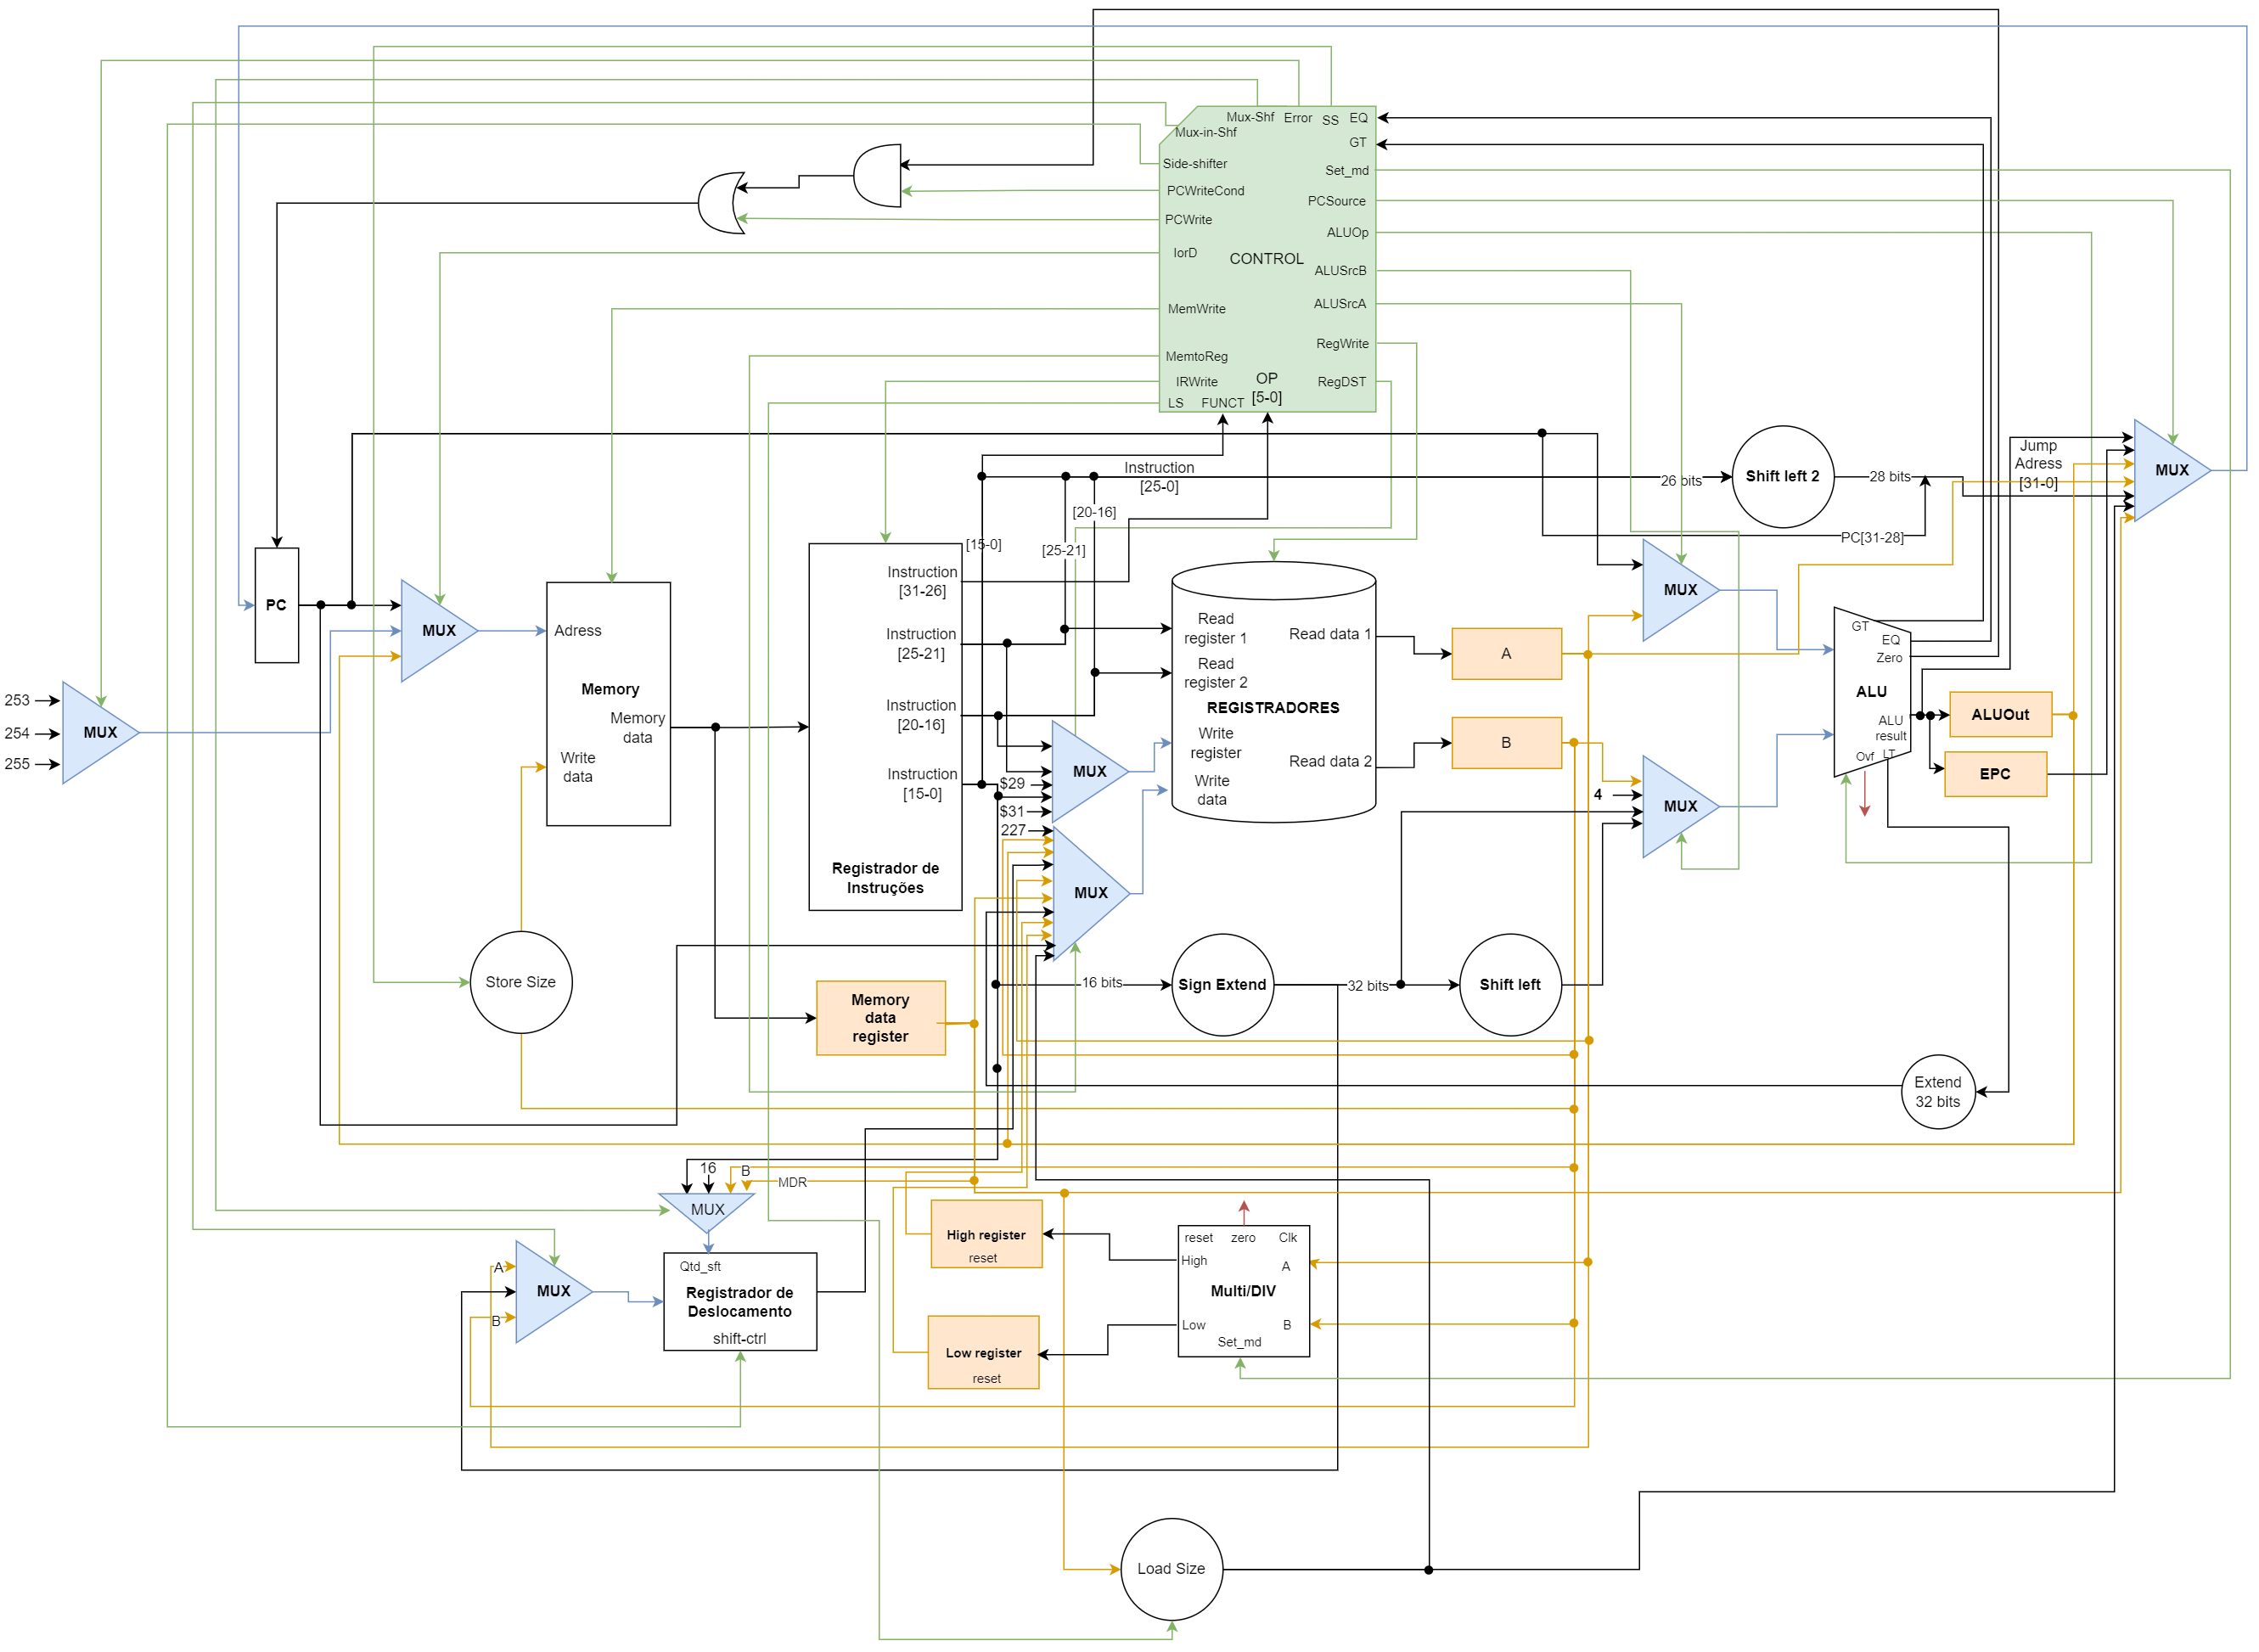
\includegraphics[width=1\textwidth]{figure/diagrama_bloco.png}
\caption{Diagrama de blocos} 
\label{fig:diagrama_blocos}
\end{figure}

A figura apresentada reflete a estrutura da unidade de processamento, onde as unidades estão representadas por blocos e as conexões por fios.

\newpage

\section{Descrição das entidades}

\subsection{load\_size}

\textbf{Inputs:}

\begin{enumerate}
    \item ls\_crtl (2 bits): Indica o tamanho da palavra carregada.
    \item data\_in (32 bits): Recebe o fio do registrador MDR.
\end{enumerate}

\textbf{Outputs:}

\begin{enumerate}
    \item data\_out (32 bits): Retorna apenas a parte do valor de MDR requerida pelo ls\_crtl concatenada com bits 0.
\end{enumerate}

\textbf{Objetivo:} Transforma os dados de 32 bits que vêm da memória em dados do tamanho necessário (32, 16 ou 8 bits) e envia-os ao banco de registradores. Num caso de exceção, ele retorna 32 bits.

\textbf{Algoritmo:} Caso o ls\_crtl seja 00 retorna os 32 bits, caso seja 01 retorna os 16 bits menos significativos concatenados com 16 bits 0, caso seja 10 retorna os 8 bits menos significativos concatenados com 24 bits 0 e caso seja 11 retorna 32 bits 0.



\subsection{xtend\_to\_32}

\textbf{Inputs:}

\begin{enumerate}
    \item Data\_in (1 bits): Recebe ULA\_LT;

\end{enumerate}

\textbf{Outputs:}

\begin{enumerate}
    \item data\_out (32 bits): Retorna o Data\_in estendido.
\end{enumerate}

\textbf{Objetivo:} Transforma o bit do fio ULA\_LT em um fio de 32 bits.

\textbf{Algoritmo:} Concatena 31 bits 0 com o valor de Data\_in.

\newpage

\subsection{shift\_left\_two}

\textbf{Inputs:}

\begin{enumerate}
    \item PC\_in (32 bits): Recebe fio do PC\_out;
    \item RS (5 bits): Recebe fio do RS;
    \item RT (5 bits): Recebe fio do RT;
    \item OFFSET (16 bits): Recebe fio do OFFSET;

\end{enumerate}

\textbf{Outputs:}

\begin{enumerate}
    \item data\_out (32 bits): Retorna o fio selecionado.
\end{enumerate}

\textbf{Objetivo:} Multiplicar por 4 o valor inserido para ser obtido o valor da instrução a ser pulada.

\textbf{Algoritmo:} Recebe os 26 bits menos significativos da instrução, dá um shift left 2 e concatena com os 4 bits mais significativos de PC\_out.


\subsection{shift\_left}

\textbf{Inputs:}

\begin{enumerate}
    \item data\_in (32 bits): Recebe o fio do XTEND\_out.

\end{enumerate}

\textbf{Outputs:}

\begin{enumerate}
    \item data\_out (32 bits): Retorna o shift left 2 da entrada.
\end{enumerate}

\textbf{Objetivo:} Dá um shift left no sinal do estendido do offset.

\textbf{Algoritmo:} Recebe o sinal do data\_in e dá um shift left 2.

\newpage

\subsection{sign\_xtend}

\textbf{Inputs:}

\begin{enumerate}
    \item data\_in (16 bits): Recebe o fio do OFFSET.

\end{enumerate}

\textbf{Outputs:}

\begin{enumerate}
    \item data\_out (32 bits): Retorna o OFFSET estendido para 32 bits.
\end{enumerate}

\textbf{Objetivo:} Estende o sinal do offset de 16 bits para 32 bits.

\textbf{Algoritmo:} Concatena 16 bits com o valor do bit mais significativo do offset com o resto do offset.



\subsection{store\_size}

\textbf{Inputs:}

\begin{enumerate}
    \item ss\_crtl (2 bits): Recebe o sinal de controle;
    \item data\_in (16 bits): Recebe o fio do REG\_B\_out.

\end{enumerate}

\textbf{Outputs:}

\begin{enumerate}
    \item data\_out (32 bits): Retorna uma parte cortada do data\_in.
\end{enumerate}

\textbf{Objetivo:} Transforma o valor do fio de saída Reg B num tamanho adequado para a memória.

\textbf{Algoritmo:} Caso o sinal de controle seja 00 retorna os 32 bits da entrada, caso seja 01 retorna 16 bits 0 com 16 bits da entrada, caso seja 10 retorna 24 bits 0 com 8 bits da entrada e, caso seja 11 retorna 32 bits 0.

\newpage

\subsection{multi\_div}

\textbf{Inputs:}

\begin{enumerate}
    \item clk (1 bit): Clock do registrador;
    \item set\_md (1 bit): Sinal de controle que escolhe a operação, 1 para divisão e 0 para multiplicação;
    \item reset (1 bit): Sinal de reset da unidade de controle;
    \item data\_a (32 bits): Valor do dividendo na divisão e multiplicando na multiplicação;
    \item data\_b (32 bits): Valor do divisor na divisão e multiplicador na multiplicação;
    \item start (1 bit): Sinal de controle da unidade de controle.
\end{enumerate}

\textbf{Outputs:}

\begin{enumerate}
    \item out\_high (32 bits): Resultado da parte maior que 32 bits na multiplicação e resto na divisão.
    \item out\_low (32 bits): Resultado da parte menor que 32 na multiplicação e quociente na divisão.
    \item zero (1 bit): Retorna 1 caso tente dividir por 0.
\end{enumerate}

\textbf{Objetivo:} Essa entidade recebe às saídas dos registradores A e B e executa a operação escolhida pela unidade de controle. O seu resultado é posteriormente armazenado nos registradores High e Low para futuras operações.

\textbf{Algoritmo:} Como decidimos por criar uma única entidade para multiplicação e divisão utilizamos respectivamente 2 algoritmos, o algoritmo de Booth para a multiplicação por complemento a dois que utiliza 32 ciclos para multiplicar os números e um algoritmo para divisão binário sem sinal que utiliza 1 ciclo para examinar e atualizar os valores dos sinais e como isso afetará o resultado e 32 ciclos para dividir, ambos algoritmos foram baseados no livro Arquitetura e Organização de Computadores \cite{arquiteturaDeComputadores}. \\

Começando pelo algoritmo de Booth, nele utilizamos 6 registradores auxiliares mult\_aux (65 bits), A (32 bits), Q (32 bits) e q\_minus\_one (1 bit), M (32 bits) e M\_negative (32 bits), onde mult\_aux é utilizado para executar o right\_sifht\_aritmética, A é o acumulador, Q é o multiplicando, M o multiplicador e M\_negative o complementeo de 2 de M e o resultado das multiplicações aparecem nos registradores A e Q, além disso, A e q\_minux\_one são inicializados em 0. \\

Segundo o autor, "A lógica de controle verifica os bits do multiplicador um de cada vez. Agora, à medida que cada bit é examinado, o bit à sua direita também é examinado. Se os dois bits forem iguais (1–1 ou 0–0), então todos os bits dos registradores A, Q e Q–1 são deslocados à direita por 1 bit. Se os dois bits forem diferentes, então o multiplicando é somado ou subtraído do registrador A, dependendo se os dois bits forem 0–1 ou 1–0. Após a adição ou subtração, ocorre o deslocamento à direita. De qualquer forma, o deslocamento à direita é tal que o bit mais à esquerda de A, a saber, An–1, não apenas é deslocado para An–2, mas também permanece em An–1. Isso é exigido para preservar o sinal do número em A e Q. Esse é conhecido como um deslocamento aritmético, pois preserva o bit de sinal." Essas operações são executadas por 32 ciclos, atualizando o valor dos registradores auxiliar e, no último ciclo, o resultado é gravado nas saidas High e Low. \\

Já para o algoritmo de divisão binária utilizamos 9 registradores auxiliares acumulator\_div (32 bits), div\_aux (64 bits), complemento\_2\_div (32 bits), data\_a\_aux\_div (32 bits), data\_b\_aux\_div (32 bits), inverter\_quociente (1 bit), inverter\_resto (1 bit), dividendo (32 bits) e divisor (32 bits), onde acumulator\_div é o acumulador, div\_aux (64 bits) é utilizado para executar o left\_shift, complemento\_2\_div é o complemento de 2 do divisor, data\_a\_aux\_div e data\_b\_aux\_div são auxiliares para inverter o sinal, inverter\_quociente e inverter\_resto são sinais de controle para inverter os valores no final e dividendo e divisor são exetamente o que se chamam. \\

Segundo o autor: "O divisor é colocado no registrador M, o dividendo no registrador Q. Em cada etapa, os registradores A e Q juntos são deslocados à esquerda por 1 bit. M é subtraído de A para determinar se A divide o resto parcial. Nesse caso, então Q0  recebe um bit 1. Caso contrário, Q0 recebe um bit 0 e M precisa ser somado de volta a A para restaurar o valor anterior. O contador é então decrementado e o processo continua por n etapas. Ao final, o quociente está no registrador Q e o resto está no registrador A" Na nossa implementação, podemos tratar M como o registrador auxiliar divisor e A e Q como sendo respectivamente acumulator\_div e dividendo. \\

O algoritmo para analisar os valores de entrada e tratar a sua saida com base nos sinais foi feito conforme as Notas do Professor Wang Jian-Sheng \cite{notasprofessor} e a implementação foi feita da seguinte forma: os valores de data\_a e data\_b são analisados e caso ambas entradas forem negativas, é armazenado o complemento de 2 de seus valores em data\_a\_aux\_div e data\_b\_aux\_div, essas variáveis auxiliares são utilizadas no algoritmo e no final e o valor do resto é invertido, caso data\_a for negativa e data\_b for positiva é armazenado em data\_a\_aux\_div o complemento de 2 de data\_a e no final são invertidos ambos restos e quocientes, já quando data\_a é positiva e data\_b é negativa é armazenado em data\_b\_aux\_div o complemento de 2 de data\_b e no final apenas o quociente é invertido.

\newpage

\subsection{REG\_A}

\textbf{Inputs:}

\begin{enumerate}
    \item Clk (1 bit): Clock do registrador;
    \item Reset (1 bit): Sinal de reset da unidade de controle;
    \item Load (1 bit): Sinal de controle da unidade de controle;
    \item Entrada (32 bits): Vetor de bits do fio de saída A do banco de registradores que carrega o registrador.
\end{enumerate}

\textbf{Outputs:}

\begin{enumerate}
    \item Saida (32 bits): Vetor de bits que possui a informação já carregada no registrador.
\end{enumerate}

\textbf{Objetivo:} Essa entidade recebe a saída A do banco de registrador e a armazena para operações futuras.

\textbf{Algoritmo:} Quando a entrada do Load é 1 e ocorre uma excitação no clock o vetor de Saida armazenado na memória se torna o vetor de entrada (o valor é atualizado). Caso o sinal de reset seja ativado, o valor da saída vira zero.

\subsection{REG\_B}

\textbf{Inputs:}

\begin{enumerate}
    \item Clk (1 bit): Clock do registrador;
    \item Reset (1 bit): Sinal de reset da unidade de controle;
    \item Load (1 bit): Sinal de controle da unidade de controle;
    \item Entrada (32 bits): Vetor de bits do fio de saída B do banco de registradores que carrega o registrador.
    
\end{enumerate}

\textbf{Outputs:}

\begin{enumerate}
    \item Saida (32 bits): Vetor de bits que possui a informação já carregada no registrador.
\end{enumerate}

\textbf{Objetivo:} Essa entidade recebe a saída B do banco de registrador e a armazena para operações futuras.

\textbf{Algoritmo:} Quando a entrada do Load é 1 e ocorre uma excitação no clock o vetor de Saida armazenado na memória se torna o vetor de entrada (o valor é atualizado). Caso o sinal de reset seja ativado, o valor da saída vira zero.

\newpage

\subsection{REG\_HIGH}

\textbf{Inputs:}

\begin{enumerate}
    \item Clk (1 bit): Clock do registrador;
    \item Reset (1 bit): Sinal de reset da unidade de controle;
    \item Load (1 bit): Sinal de controle da unidade de controle;
    \item Entrada (32 bits): Vetor de bits do fio de saída High da entidade mult/div que carrega o registrador.
\end{enumerate}

\textbf{Outputs:}

\begin{enumerate}
    \item Saida (32 bits): Vetor de bits que possui a informação já carregada no registrador.
\end{enumerate}

\textbf{Objetivo:} Essa entidade recebe a saída High do mult/div e a armazena para operações futuras.

\textbf{Algoritmo:} Quando a entrada do Load é 1 e ocorre uma excitação no clock o vetor de Saida armazenado na memória se torna o vetor de entrada (o valor é atualizado). Caso o sinal de reset seja ativado, o valor da saída vira zero.



\subsection{REG\_LOW}

\textbf{Inputs:}

\begin{enumerate}
    \item Clk (1 bit): Clock do registrador;
    \item Reset (1 bit): Sinal de reset da unidade de controle;
    \item Load (1 bit): Sinal de controle da unidade de controle;
    \item Entrada (32 bits): Vetor de bits do fio de saída Low da entidade mult/div que carrega o registrador.
    
\end{enumerate}

\textbf{Outputs:}

\begin{enumerate}
    \item Saida (32 bits): Vetor de bits que possui a informação já carregada no registrador.
\end{enumerate}

\textbf{Objetivo:} Essa entidade recebe a saída Low do mult/div e a armazena para operações futuras.

\textbf{Algoritmo:} Quando a entrada do Load é 1 e ocorre uma excitação no clock o vetor de Saida armazenado na memória se torna o vetor de entrada (o valor é atualizado). Caso o sinal de reset seja ativado, o valor da saída vira zero.

\newpage

\subsection{REG\_EPC}

\textbf{Inputs:}

\begin{enumerate}
    \item Clk (1 bit): Clock do registrador;
    \item Reset (1 bit): Sinal de reset da unidade de controle;
    \item Load (1 bit): Sinal de controle da unidade de controle;
    \item Entrada (32 bits): Vetor de bits do fio de saída ULA\_RESULT da ULA que carrega o registrador.
    
\end{enumerate}

\textbf{Outputs:}

\begin{enumerate}
    \item Saida (32 bits): Vetor de bits que possui a informação já carregada no registrador.
\end{enumerate}

\textbf{Objetivo:} Essa entidade recebe a saída do resultado da ULA e a armazena para ser utilizada pelo MUX PC\_Source.

\textbf{Algoritmo:} Quando a entrada do Load é 1 e ocorre uma excitação no clock o vetor de Saida armazenado na memória se torna o vetor de entrada (o valor é atualizado). Caso o sinal de reset seja ativado, o valor da saída vira zero.



\subsection{REG\_ALU\_OUT}

\textbf{Inputs:}

\begin{enumerate}
    \item Clk (1 bit): Clock do registrador;
    \item Reset (1 bit): Sinal de reset da unidade de controle;
    \item Load (1 bit): Sinal de controle da unidade de controle;
    \item Entrada (32 bits): Vetor de bits do fio de saída ULA\_RESULT da ULA que carrega o registrador.
    
\end{enumerate}

\textbf{Outputs:}

\begin{enumerate}
    \item Saida (32 bits): Vetor de bits que possui a informação já carregada no registrador.
\end{enumerate}

\textbf{Objetivo:} Essa entidade recebe a saída do resultado da ULA e a armazena para operações futuras.

\textbf{Algoritmo:} Quando a entrada do Load é 1 e ocorre uma excitação no clock o vetor de Saida armazenado na memória se torna o vetor de entrada (o valor é atualizado). Caso o sinal de reset seja ativado, o valor da saída vira zero.
\newpage

\subsection{MEM\_DATA\_REG}

\textbf{Inputs:}

\begin{enumerate}
    \item Clk (1 bit): Clock do registrador;
    \item Reset (1 bit): Sinal de reset da unidade de controle;
    \item Load (1 bit): Sinal de controle da unidade de controle;
    \item Entrada (32 bits): Vetor de bits do fio de saída da entidade de memória que carrega o registrador.
\end{enumerate}

\textbf{Outputs:}

\begin{enumerate}
    \item Saida (32 bits): Vetor de bits que possui a informação já carregada no registrador.
\end{enumerate}

\textbf{Objetivo:} Essa entidade recebe a saída do resultado da memória e a armazena para operações futuras.

\textbf{Algoritmo:} Quando a entrada do Load é 1 e ocorre uma excitação no clock o vetor de Saida armazenado na memória se torna o vetor de entrada (o valor é atualizado). Caso o sinal de reset seja ativado, o valor da saída vira zero.

\newpage

\section{Descrição das Operações}

As operações são classificadas em R,I e J. Que são referentes aos formatos das instruções e às operações que podem ser realizadas pelo MIPS. Todas elas, antes de serem executadas, passam pelo momento de Fetch e de Decode, para ler a instrução e decodificá-la.

\subsection{Fetch}

O valor de PC é somado com o número 4 na ULA, e o resultado é armazenado em ALUOut. Após isso, esse valor é passado pelo Mux e escrito no registrador PC, que guardará esse valor enquanto a unidade de leitura de instruções está desativada devido à execução de outra no mesmo momento.

\subsection{Decode}

O valor em PC é lido pela memória e passado para o Intruction Register, para poder ser decodificado e separar seus bits entre OPCODE, RS, RT e os últimos 16 bits que variam conforme o tipo de instrução, deixando tudo preparado para a execução das próximas instruções.

%O valor imediato (IMMEDIATE) é estendido para 32 bits pelo SignExtend, e esse valor, junto com o valor de PC, são enviados para a ULA para realizar uma operação de soma. O resultado é armazenado em ALUOut. No próximo ciclo de clock, o registrador A é carregado com o valor de Read Data 1 e o registrador B é carregado com o valor de Read Data 2, ambos provenientes da entidade de registradores. Enquanto isso, é realizado um "case" para determinar qual é a instrução atual.

\newpage

 \subsection{R}
 
Operações do tipo R são usadas principalmente para operações aritméticas e lógicas entre os registradores. Elas possuem o formato que inclui campos para três registradores de origem (rs, rt, rd), um campo para deslocamento (shampt) e um campo para função (funct).

 \subsubsection{Campos da instrução R}

 \begin{enumerate}
    \item Opcode: Identifica a operação que irá ser executada, para os tipos R o opcode é zero (0);
    \item Registradores de origem (rs,rt): Eles indicam os registradores que contêm os operandos para a operação. Para uma adição, o rs pode conter o primeiro operando e rt pode conter o segundo operando, por exemplo;
    \item Registradores de destino (rd): Indica o registrador onde o resultado da operação será armazenado. Após a operação, o resultado será colocado no rd;
    \item Deslocamento (shampt): Em algumas instruções, como o deslocamento lógico (sll) ou deslocamento à direita (srl) este campo é usado para especificar quantos bits serão deslocados;
    \item Função (funct): Identifica a operação a ser realizada dentro do conjunto de operações pelo opcode.
\end{enumerate}

 \subsubsection{ADD, SUB e AND}

As três instruções fazem operações diferentes com os valores dos registradores A e B e colocam o resultado em rd. ADD faz soma, SUB subtração e AND realiza um and lógico bit a bit dos valores. Os valores de A e B são carregados pela ALU e a operação ocorre segundo o funct, depois o resultado é armazenado no ALUOut e é guardado no registrador apenas no próximo ciclo, sendo diferente apenas para o AND, onde o valor de saída é o fio EQ da unidade de controle, ele será entendido para 32 bits e salvo no registrador rd.

 \subsubsection{DIV e MULT}
 
DIV faz a divisão e MULT a multiplicação, guardando o resultado em LO e HI. Os valores de A e B são passados para o bloco MULT/DIV e a operação é realizada, resultando em saídas high e low, que no mult significa os 32 bits mais significativos e os 32 bits menos significativos. No div o high é o resto e o low é o quociente. Eles então são carregados nos registradores High e Low.

 \subsubsection{JR}

Armazena o endereço contido no registrador rs (Normalmente o 31) no PC, fazendo o código continuar a partir da linha contida no registrador passado, muito utilizado em chamadas de funções.

 \subsubsection{MFHI e MFLO}
 
As duas instruções pretendem gravar o conteúdo dos registradores HI ou LO, respectivamente, no registrador rd. Durante o funcionamento dessas instruções, o valor armazenado no registrador HI ou LO, dependendo da instrução executada, é transferido para o registrador especificado por rd. 

\subsubsection{SLL, SRA e SRL}

As três instruções têm como objetivo armazenar no registrador rd o valor do registrador B deslocado em um número específico de unidades à direita ou à esquerda, conforme determinado pela instrução. O deslocamento shamt é extraído dos bits 10 a 6 da instrução, definindo assim o valor N, ou seja, o número de unidades a serem deslocadas. O valor do registrador B é então enviado através do multiplexador juntamente com o valor N para o Registrador de Deslocamento, onde ocorre o deslocamento adequado, onde levará um ciclo para ser escrito no Registrador de Deslocamento e um para deslocar. No próximo ciclo de clock, o resultado do deslocamento é armazenado no registrador rd. O código de deslocamento para a instrução SLL é 010, para SRA é 100 e para SRL é 011.

\subsubsection{SLLV e SRAV}

Armazena no registrador rd o valor do registrador A deslocado em um número específico de unidades à esquerda ou à direita, conforme determinado pela instrução. Durante o funcionamento dessas instruções, o valor do registrador B é enviado ao multiplexador, que fornecerá o deslocamento de B unidades ao registrador A. Simultaneamente, o valor do registrador A é encaminhado ao multiplexador. Ambos os valores, após passarem pelos seus respectivos multiplexadores, são direcionados para o Registrador de Deslocamento, onde serão salvos e o deslocamento será realizado consoante o código de deslocamento (SLLV é 010, SRAV é 100). No próximo ciclo de clock, a saída resultante do deslocamento é armazenada no registrador rd.

\subsubsection{SLT}

Compara dois valores armazenados nos registradores A e B e determina se A é maior que B, armazenando o resultado da comparação em rd. Durante o funcionamento dessa instrução, os valores armazenados nos registradores A e B são enviados para a ALU, onde ocorre a operação de comparação. Se A for maior que B, a saída da ALU para esta operação, chamada GT, será 1; caso contrário, será 0. Esta saída GT, que possui apenas um bit (0 ou 1), é então expandida para 32 bits mediante um processo chamado sign extend. Em seguida, o valor expandido é escrito no registrador rd do banco de registradores, indicando o resultado da comparação entre A e B.

\subsubsection{BREAK}

Realiza uma subtração entre o valor atual do contador de programa (PC) e o valor 4, e então escreve o resultado de volta no PC. O valor atual do PC é enviado para um multiplexador, enquanto o valor 4 é enviado para outro multiplexador. Ambos os valores são então encaminhados para a Unidade Lógico-Aritmética (ALU), onde ocorre a operação de subtração. O resultado da subtração, ou seja, o valor do PC subtraído por 4, é então selecionado pelo multiplexador e escrito de volta no registrador do contador de programa (PC). Essa operação resulta na atualização do valor do PC, preparando-o para a próxima instrução a ser executada.

\subsubsection{RTE}

Carrega o valor do registrador EPC em PC. O valor do registrador EPC passa por Mux PC e é carregado em PC.

\subsubsection{XCHG}

Faz a leitura dos valores de rs e rt e troca. Ou seja, o valor de rs vai para rt e o valor de rt vai para rs.

\newpage

\subsection{I}

Possui um formato que inclui um opcode, dois campos para os registradores de origem (rs e rt) e um campo para o valor imediato (immediate). O campo de valor imediato é usado para fornecer um dado constante ou um endereço de memória, dependendo do contexto da instrução.

\subsubsection{ADDI e ADDIU}

ADDIU (Add Immediate Unsigned) soma o valor imediato (IMMEDIATE), estendido para 32 bits, com o conteúdo do registrador A. A diferença em relação ao ADDI é que o ADDIU ignora exceções de overflow. Durante a operação, o valor do registrador A é enviado para a ALU, onde é somado ao IMMEDIATE após este ter sido estendido para 32 bits pelo sign extend. O resultado da soma é então armazenado em ALUOut e, no próximo ciclo de clock, é transferido para o registrador rt.

\subsubsection{BEQ e BNE}

BEQ (Branch if Equal) compara os valores dos registradores A e B. Se eles forem iguais, a flag EQ é definida como 1, caso contrário, a flag EQ é definida como 0. Essa flag é enviada para a unidade de controle, que por sua vez informa que haverá desvio e passará os sinais corretos para os módulos passarem o valor do desvio, calculado previamente, para o PC. No caso do BEQ, ele desvia em casos de igualdade e o BNE em casos de desigualdades (!==).

\subsubsection{BLE e BGT}

Compara os valores nos registradores A e B na ALU. Se A for maior que B, a flag GT é definida como 1; caso contrário, é definida como 0. Essas flags são enviadas para a unidade de controle, que por sua vez informa que haverá desvio e passará os sinais corretos para os módulos passarem o valor do desvio, calculado previamente, para o PC. No caso do BLE ele desvia no caso de A ser menor ou igual a B e o BGT caso A seja maior que B.

%Troquei por estar igual ao relatório do drive, tinha até as comparações

\subsubsection{LB, LH e LW}

Calcula a soma da extensão do offset para 32 bits com o valor contido no registrador rs, e então armazena esse resultado no registrador rt. Durante o funcionamento da instrução, o offset é estendido para 32 bits por meio do sign extend e somado ao valor armazenado no registrador A. O resultado dessa soma é então enviado para a memória, onde seu correspondente é armazenado no Registrador de Dados da Memória (Memory Data Register). Em seguida, esse valor passa pelo seletor Load Size, que determina o tamanho da palavra a ser armazenada. Se o seletor indicar LB, o tamanho da palavra é de 1 byte (00); se for LH, o tamanho é de 2 bytes (01); e se for LW, o tamanho é de 4 bytes (10). Finalmente, o valor é gravado no endereço especificado pelo registrador rt.

\subsubsection{LUI}

Realiza um deslocamento para a esquerda de 16 bits no valor imediato (IMMEDIATE) contido nos bits [15:0] do registrador de instruções. Isso significa que o valor é estendido para 32 bits, adicionando 16 zeros à direita. Em seguida, esse valor estendido é armazenado no registrador rt do banco de registradores.

\subsubsection{SB, SH e SW}

Calcula o endereço de memória que será armazenado a partir da soma do offset e do valor do registrador rt, a partir do valor encontrado nesse endereço, faz o "corte" dos bits que serão armazenados, pegando apenas o Byte, metade (Half) ou o valor completo que será inserido nesse endereço pela unidade de memória da CPU.

%Calcula a soma da extensão do offset para 32 bits com o valor contido no registrador rs e armazena um certo tamanho do registrador rt no endereço de memória determinado por essa soma. Durante o funcionamento da instrução, o offset é estendido para 32 bits por meio do sign extend e somado ao valor armazenado no registrador A. A soma resultante é armazenada em ALUOut e, no próximoS ciclo, é enviada para a memória através do endereço e gravada no Registrador de Dados da Memória. O valor do registrador B é então armazenado nesse endereço, e o tamanho da palavra a ser gravada é determinado pelo seletor Store Size. Se o seletor for 00, apenas 1 byte é armazenado (Store Byte); se for 01, metade da palavra é armazenada (Store Half-Word); e se for SW, a palavra inteira é armazenada sem passar pelo Store Size.

\subsubsection{SLTI}

Compara o valor armazenado no registrador A com um valor imediato para determinar se A é maior que o imediato. Durante o funcionamento da instrução, o valor imediato é estendido de 16 para 32 bits por meio do sign extend. Em seguida, tanto o valor do registrador A quanto o valor imediato são enviados para a ALU, onde é realizada a operação de comparação. Se A for maior que o imediato, a saída GT da ALU é 1; caso contrário, é 0. Essa saída é então estendida de 1 para 32 bits antes de ser retornada para o banco de registradores e armazenada no registrador RT.

\subsubsection{SRAM}

Durante o primeiro ciclo de clock, os valores dos registradores rs e rt são lidos. Em seguida, o endereço de memória é calculado na ULA com base no valor de rt. No próximo ciclo de clock, o valor correspondente é lido na memória e armazenado no Memory Data Register. Após isso, o valor do registrador rs é deslocado n vezes pelo valor lido da memória, e o resultado é escrito de volta no registrador rs.

\newpage

\subsection{J}

São utilizadas para realizar desvios incondicionais no código, ou seja, alterar o fluxo de execução do programa sem depender de condições.

\subsubsection{J}

Salta para uma parte específica do código, opera concatenando os bits 0 a 25 do Registrador de Instrução para obter o deslocamento. Em seguida, esse valor é deslocado para a esquerda e concatenado com os 4 bits mais significativos do Contador de Programa (PC), resultando em um valor de 32 bits então gravado no PC. Isso permite que o programa pule para a parte desejada do código.

 \subsubsection{JAL}

Pula para uma parte específica do código e guarda o valor de PC+4 (a próxima instrução a ser executada), primeiro calcula o valor de PC+4 e armazena em ALUOut. Em seguida, concatena os bits de 0 a 25 do Registrador de Instrução para obter o deslocamento, faz um deslocamento para a esquerda nesse valor e ainda concatena com os 4 bits mais significativos do PC. O valor resultante, de 32 bits, é então gravado no PC. Por fim, o valor de ALUOut é armazenado no registrador de número 31.

 \subsection{Tratamento de Erros}
 
Escreve o valor da Instrução que deu erro no registrador EPC, depois irá ver qual o erro e puxará da memória um endereço (Opcode, Overflow e div0). Lê essa memória e escreve no Memory Data Register(MDR), depois escreve o valor em PC.
 
\newpage

\section{Descrição dos Estados do Controle}

\subsection{ADD, SUB e AND}
Durante o primeiro ciclo, a CPU identifica a operação a ser realizada e lê os valores dos registradores rt e rs no banco de registradores. Esses valores são então escritos nos registradores A e B, respectivamente. No segundo ciclo, a ULA executa a operação especificada (Adição, subtração e AND), verificando o overflow, e o resultado é armazenado no registrador AluOut. No último ciclo, o valor contido no registrador AluOut é escrito de volta no registrador rs.

\subsection{MULT e DIV}

No primeiro ciclo, os valores de rt e rs são escritos nos registradores A e B e passando para o mult/div, do segundo ciclo até o 35 (se for mult) ou do segundo ciclo até o 36 (se for div) os valores são inscritos no hi e lo, no qual o hi é o resto e lo o quociente para as divisões. Para a mult, hi são os 32 bits mais significativos e o lo os 32 bits menos significativos.

\subsection{JR}

No primeiro ciclo de clock o registrador rs é lido e seu valor escrito no registrador A, após isso, no segundo ciclo o valor é passado para o registrador PC, que irá continuar a execução do código a partir da linha de execução contida no registrador rs.


\subsection{MFHI e MFLO}

Os valores de HI e LO são escritos no RD, levando apenas um ciclo.

\subsection{SLL, SRA e SRL}

No primeiro ciclo o registrador RT é lido e escrito em B e é direcionado para a entrada, enquanto o valor de shamt (valor de deslocamento) é direcionado para N (Ambas entradas do Regsitrador de Deslocamento). No próximo ciclo de clock, o valor de shift é configurado para salvar os valores e depois o valor de shift é setado de acordo com a instrução (Deslocamento lógico, áritimétrico para direita ou esquerda). Enquanto isso, o valor do registrador rd é direcionado para o registrador de destino (Write Register), e a saída do registrador de deslocamento é direcionada para os dados a serem escritos (Write Data), ambos localizados na entidade do registrador. Este ciclo completa o processo de deslocamento e escrita de dados.

\subsection{SLLV e SRAV}

No primeiro ciclo de clock, os valores dos registradores A e B são lidos e no segundo são redirecionados para a "entrada" e "N", respectivamente (Do Registrador de Deslocamento), enquanto o shift é configurado para carregar os valores no registrador de deslocamento. No próximo ciclo de clock, o shift é ajustado. Além disso, os valores dos registradores de destino (rd) e a saída do registrador de deslocamento são direcionados para o registrador de destino (Write Register) e os dados a serem escritos (Write Data), respectivamente, na entidade do registrador. No terceiro ciclo de clock, o shift é configurado como 000 para evitar cálculos errados e preparar o sistema para as próximas operações.

\subsection{SLT}

No primeiro ciclo de clock, os valores dos registradores A e B são direcionados para a ULA, enquanto a operação da ULA é configurada como 111 para realizar uma operação de comparação. No próximo ciclo de clock, o valor do rd é direcionado para o registrador de destino (Write Register), enquanto a saída do SignExtend, que é uma extensão de sinal de 1 para 32 bits, é direcionada para os dados a serem escritos (Write Data), ambos localizados na entidade do registrador. Neste ciclo, o valor resultante da comparação é escrito no registrador de destino (RD) com Reg\_WR = 1.

\subsection{Break}

No primeiro ciclo de clock, o sinal do PC e o valor 4 são direcionados para a ULA, enquanto a operação da ULA é configurada como 010 para realizar uma operação de subtração. No próximo ciclo de clock, o resultado da subtração é direcionado de volta para o PC, e a sinalização PCWrite é ativada, permitindo que o valor do Program Counter seja atualizado com o resultado da subtração.

\subsection{RTE}

O valor do registrador EPC é direcionado até PC.

\subsection{ADDI e ADDIU}

Durante o primeiro ciclo de clock, o valor do IMMEDIATE é direcionado para o bloco de extensão de sinal (SignExtend) para ser convertido de 16 para 32 bits e o valor do registrador é lido e escrito no registrador A. Este valor estendido e o valor do registrador No ciclo seguinte, os valores são então direcionados para a ULA, configurada para realizar uma operação de soma=001, e o resultado é armazenado em ALUOut. No próximo ciclo de clock, no caso de uma instrução do tipo ADDI, uma análise é realizada para determinar se a soma resultou em um overflow; se não houver overflow, o valor é escrito no registrador RT com o sinal de escrita no registrador Reg\_WR. Lembrando que o ADDI retorna overflow e o ADDIU não retorna.

\subsection{BEQ, BNE, BLE e BGT}

Os valores de rs e rt são lidos e escritos em A e B, enquanto isso o valor do desvio é calculado e armazenado no ALUOut para caso o desvio se confirme. No ciclo seguinte o valor de A e B são comparados e é verificado se houve desvio ou não. Nos casos do BEQ e BNE, para que o desvio ocorra, é nescessário que o valor de EQ seja, respectivamente, 1 ou 0. Semelhante ocorre com BLE e BGT, mas considerando o valor de GT, nesse caso os valores para que o desvio ocorresse em cada instrução são, respectivamente, 1 ou 0. Caso haja, o valor calculado anteriormente é passado para o registrador PC.

 \subsection{LW, LH e LB}

Durante o primeiro ciclo de clock, o valor do offset é estendido de 16 para 32 bits pelo bloco de extensão de sinal (SignExtend). Em seguida, esse offset estendido e o valor do registrador A são direcionados para a ULA, configurada para realizar uma operação de soma (operação 001), e o resultado é armazenado em ALUOut. No próximo ciclo de clock, o valor de ALUOut é enviado para a entrada de endereço da Memória. A leitura da memória leva 2 ciclos de clock, após o qual o valor é carregado no registrador MDR. No próximo ciclo, o valor do LoadSize é configurado. O resultado é então transferido para o registrador rt através da saída LoadSize\_Out\_Up, com o sinal de escrita no registrador (RegWR) ativado (O load size servirá para controlar o tamanho da saída).

\subsection{LUI}

No primeiro ciclo o valor do imediato é carregado no Registrador de Deslocamento e é setado para deslocar 16 vezes, após isso, no segundo ciclo acontece o deslocamento e, por fim, no terceiro, o valor é salvo no registrador RS.

\subsection{SW, SB e SH}

Durante o primeiro ciclo de clock, o valor do offset é estendido de 16 para 32 bits pelo bloco de extensão de sinal (SignExtend) e o valor do registrador rs e rt são lidos em A e B. Em seguida, esse offset estendido e o valor do registrador B são direcionados para a ULA, configurada para realizar uma operação de soma (operação 001), e o resultado é armazenado em ALUOut. No próximo ciclo de clock, o valor de ALUOut é enviado para a entrada de endereço da Memória e o valor de A é direcionado para ser escrito nesse endereço de memória, passando antes pelo store size que definirá qual será o tamanho do valor armazenado (Byte, Half ou Word)

\subsection{SLTI}

Durante o primeiro ciclo de clock, o valor do offset é estendido de 16 para 32 bits pelo bloco de extensão de sinal (SignExtend). Em seguida, esse offset estendido e o valor do registrador A são direcionados para a ULA, configurada para realizar uma operação de comparação (operação 111). Depois, o valor do registrador de destino (rt) é direcionado para o registrador de destino (Write Register), enquanto a saída do SignExtend, que é uma extensão de sinal de 1 para 32 bits, é direcionada para os dados a serem escritos (Write Data), ambos localizados na entidade do registrador. Neste ciclo, o valor resultante da comparação é escrito no registrador de destino (rt) com o sinal de escrita no registrador Reg\_WR.

\subsection{J}

O valor do offset é multiplicado por 4 pelo shift left 2 e então escolhido como fonte do endereço de PC.

\subsection{JAL}

Semelhante ao "J" o valor do offset é multiplicado por 4 e entao escolhido como fonte do endereço de PC, ao mesmo tempo que o endereço atual de PC é escrito na saída da ALU. No próximo ciclo, esse valor é carregado em write data, e o registador de destino "31" é escolhido.
 
\subsection{RESET}

Na entidade de registradores, o número 227 é escrito no registrador de número 29, com a operação de escrita habilitada, realizando um reset, todos os registradores são zerados e todos os sinais de controle também são zerados.

\subsection{Overflow, Opcode404, Div0}

O erro, quando identificado, realiza no primeiro ciclo a escrita do valor de PC em EPC e depois faz a leitura do tratamento de erro, pegando o valor 253, 254 ou 255 a depender do tipo de erro. Depois disso esse valor passa pela memória e é lido, levando 2 ciclos para isso. Logo após o valor lido é escrito no registrador MDR e é cortado o byte dele no módulo de Load Size, e passado para o registrador PC para continuar a rotina de tratamento de erros.

\subsection{Estado Comum}
 
Faz o Pc + 4 e a identificação da instrução.

\newpage

\section{Conjunto de Simulações}

\subsection{Simulações das entidades: }
\subsubsection{load\_size}
\textbf{Descrição das Portas:}

\textbf{Inputs:}

\begin{enumerate}
    \item ss\_crtl (2 bits): Recebe sinal de controle;
    \item data\_in (16 bits): Recebe o fio do REG\_B\_out.

\end{enumerate}

\textbf{Outputs:}

\begin{enumerate}
    \item data\_out (32 bits): Retorna uma parte cortada do data\_in
\end{enumerate}

\textbf{Descrição da Simulação:} Em cada ciclo temos um dos possiveis valores de controle, pode-se ver que os valores da saída data\_out são os valores da entrada data\_in tratados como esperado.

\begin{figure}[htbp!]
\centering
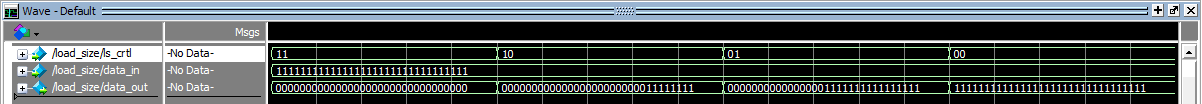
\includegraphics[width=1\textwidth]{figure/simulacao_load_size.png}
\caption{Simulação Load Size} 
\label{fig:imagem_massa}
\end{figure}

\subsubsection{xtend\_to\_32}
\textbf{Descrição das Portas:}

\textbf{Inputs:}

\begin{enumerate}
    \item Data\_in (1 bits): Recebe ULA\_LT.
\end{enumerate}

\textbf{Outputs:}

\begin{enumerate}
    \item data\_out (32 bits): Retorna o Data\_in extendido.
\end{enumerate}

\textbf{Descrição da Simulação:} Podemos ver nos 2 ciclos testados que o valor da saída data\_out é o valor de data\_in estendido.

\begin{figure}[htbp!]
\centering
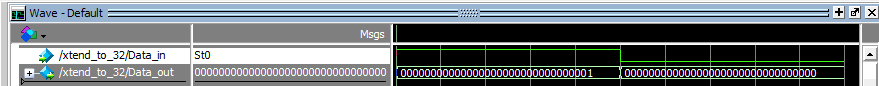
\includegraphics[width=1\textwidth]{figure/simulacao_xtend_to_32.png}
\caption{Simulação Xtend to 32} 
\label{fig:imagem_massa}
\end{figure}

\subsubsection{shift\_left\_two}
\textbf{Descrição das Portas:}

\textbf{Inputs:}

\begin{enumerate}
    \item PC\_in (32 bits): Recebe o fio do PC\_out;
    \item RS (5 bits): Recebe o fio do RS;
    \item RT (5 bits): Recebe o fio do RT;
    \item OFFSET (16 bits): Recebe o fio do OFFSET.

\end{enumerate}

\textbf{Outputs:}

\begin{enumerate}
    \item data\_out (32 bits): Retorna o fio selecionado.
\end{enumerate}

\textbf{Descrição da Simulação:} Como podemos ver, ele concatena os 26 bits menos significativos da instrução, dá um shift left 2 e concatena com os 4 bits mais significativos do pc\_in.

\begin{figure}[htbp!]
\centering
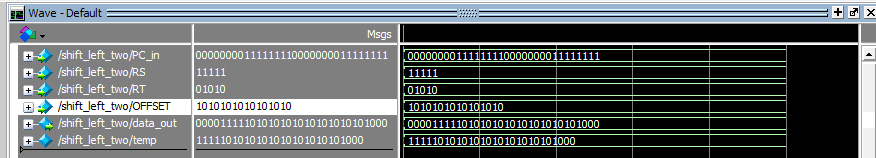
\includegraphics[width=1\textwidth]{figure/simulacao_shift_left_two.png}
\caption{Simulação Shift Left Two} 
\label{fig:imagem_massa}
\end{figure}

\subsubsection{shift\_left}
\textbf{Descrição das Portas:}

\textbf{Inputs:}

\begin{enumerate}
    \item data\_in (32 bits): Recebe fio do XTEND\_out.

\end{enumerate}

\textbf{Outputs:}

\begin{enumerate}
    \item data\_out (32 bits): Retorna o shift left 2 da entrada.
\end{enumerate}

\textbf{Descrição da Simulação:} Como podemos ver, ele dá um shift left 2 na entrada data\_in.

\begin{figure}[htbp!]
\centering
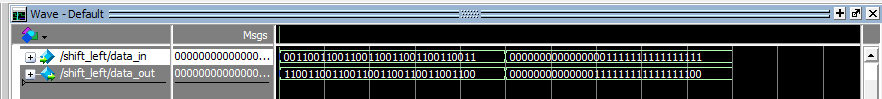
\includegraphics[width=1\textwidth]{figure/simulacao_shift_left.png}
\caption{Simulação Shift Left} 
\label{fig:imagem_massa}
\end{figure}

\subsubsection{sign\_xtend}
\textbf{Descrição das Portas:}

\textbf{Inputs:}

\begin{enumerate}
    \item data\_in (16 bits): Recebe o fio do OFFSET.

\end{enumerate}

\textbf{Outputs:}

\begin{enumerate}
    \item data\_out (32 bits): Retorna o OFFSET extendido para 32 bits.
\end{enumerate}

\textbf{Descrição da Simulação:} Como podemos ver, ele extende o bit de sinal do data\_in e transforma a entrada de 16 bits em uma saída de 32.

\begin{figure}[htbp!]
\centering
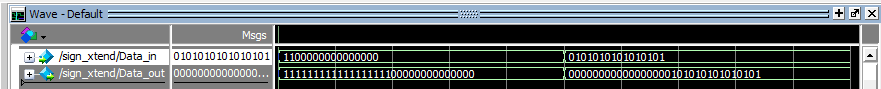
\includegraphics[width=1\textwidth]{figure/simulacao_sign_xtend.png}
\caption{Simulação Sign Xtend} 
\label{fig:imagem_massa}
\end{figure}

\subsubsection{store\_size}
\textbf{Descrição das Portas:}

\textbf{Inputs:}

\begin{enumerate}
    \item ss\_crtl (2 bits): Recebe o sinal de controle;
    \item data\_in (16 bits): Recebe o fio do REG\_B\_out.

\end{enumerate}

\textbf{Outputs:}

\begin{enumerate}
    \item data\_out (32 bits): Retorna uma parte cortada do data\_in
\end{enumerate}

\textbf{Descrição da Simulação:} Em cada ciclo temos um dos possiveis valores de controle, pode-se ver que os valores da saída data\_out são os valores da entrada data\_in tratados como esperado.

\begin{figure}[htbp!]
\centering
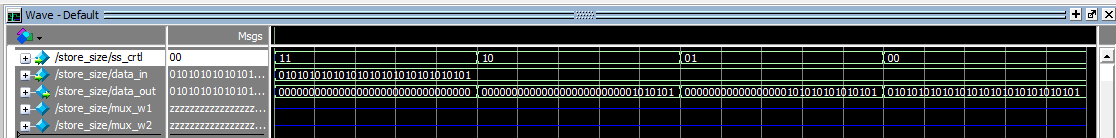
\includegraphics[width=1\textwidth]{figure/simulacao_store_size.png}
\caption{Simulação Store Size} 
\label{fig:imagem_massa}
\end{figure}

\subsubsection{multi\_div}
\textbf{Descrição das Portas:}

\begin{enumerate}
    \item clk (1 bit): Clock do registrador;
    \item set\_md (1 bit): Sinal de controle que escolhe a operação, 1 para divisão e 0 para multiplicação;
    \item reset (1 bit): Sinal de reset da unidade de controle;
    \item data\_a (32 bits): Valor do dividendo na divisão e multiplicando na multiplicação;
    \item data\_b (32 bits): Valor do divisor na divisão e multiplicador na multiplicação;
    \item start (1 bit): Sinal de controle da unidade de controle.
\end{enumerate}

\textbf{Outputs:}

\begin{enumerate}
    \item out\_high (32 bits): Resultado da parte maior que 32 bits na multiplicação e resto na divisão.
    \item out\_low (32 bits): Resultado da parte menor que 32 na multiplicação e quociente na divisão.
    \item zero (1 bit): Retorna 1 caso tente dividir por 0.
\end{enumerate}

\textbf{Descrição da Simulação:} Podemos ver nas simulações de multiplicações e divisões que os resultados foram impressos de forma correta.

\begin{figure}[htbp!]
\centering
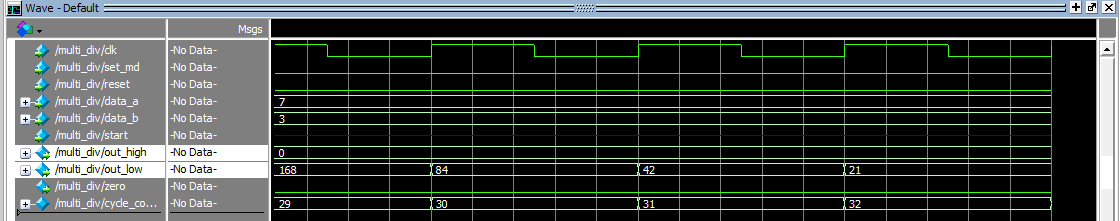
\includegraphics[width=1\textwidth]{figure/simulacao_mult_1.png}
\caption{Simulação Multi 1} 
\label{fig:imagem_massa}
\end{figure}

\begin{figure}[htbp!]
\centering
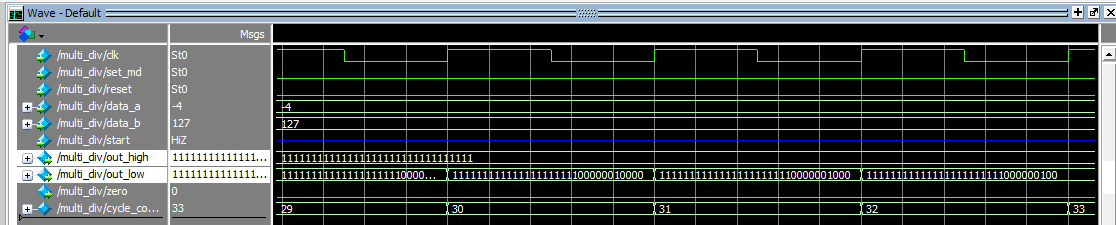
\includegraphics[width=1\textwidth]{figure/simulacao_mult_2.png}
\caption{Simulação Multi 2, valor de low é -508 em binario} 
\label{fig:imagem_massa}
\end{figure}

\begin{figure}[htbp!]
\centering
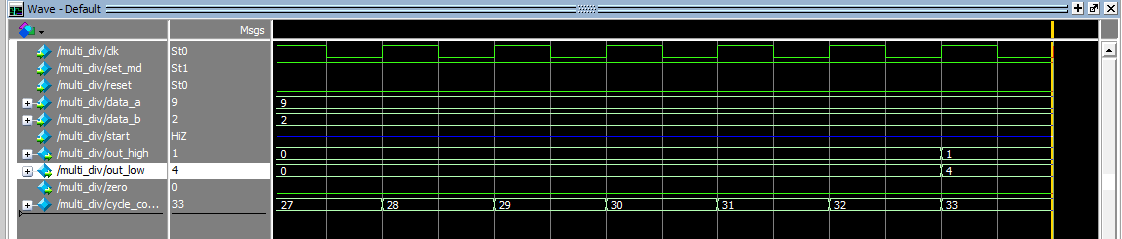
\includegraphics[width=1\textwidth]{figure/simulacao_div_1.png}
\caption{Simulação Div 1} 
\label{fig:imagem_massa}
\end{figure}

\begin{figure}[htbp!]
\centering
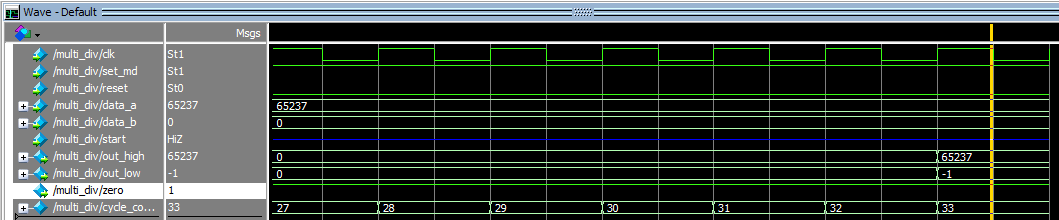
\includegraphics[width=1\textwidth]{figure/simulacao_div_2.png}
\caption{Simulação Div 2, divisão por 0} 
\label{fig:imagem_massa}
\end{figure}

\newpage

\subsection{Simulação das instruções}

\subsubsection{ADD}
\textbf{Instruções testadas:}
\lstinputlisting{codes/add.asm} \\

 \textbf{Descrição da simulação:} Será adicionado o valor 12 no registrador \$1 com o addi, o valor 8 será alocado ao registrador \$2 e depois somado e inserido no registrador \$3, o esperado é o valor 20.\\

\begin{figure}[htbp!]
\centering
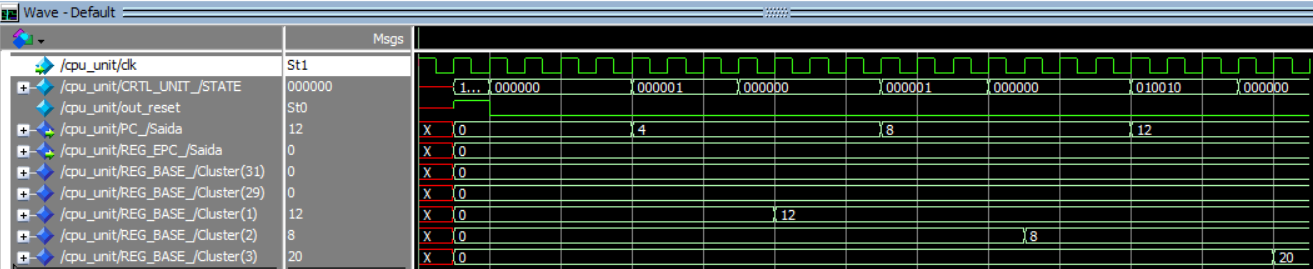
\includegraphics[width=1\textwidth]{figure/simulacao_add.png}
\caption{Simulação Add} 
\label{fig:imagem_massa}
\end{figure}

\subsubsection{SUB}
\textbf{Instruções testadas:}
\lstinputlisting{codes/sub.asm} \\

\textbf{Descrição da simulação:} Será adicionado o valor 12 no registrador \$1 com o addi, o valor 8 será alocado ao registrador \$2 e depois subtraído e inserido no registrador \$3, o esperado é o valor 4.\\

\begin{figure}[htbp!]
\centering
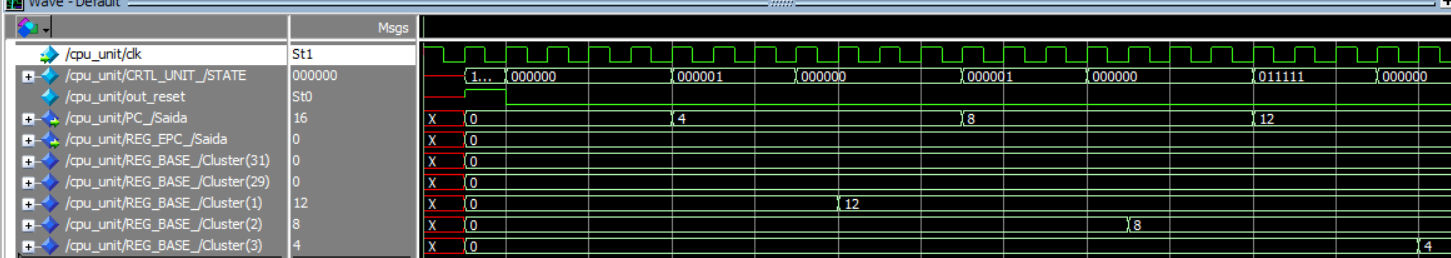
\includegraphics[width=1\textwidth]{figure/simulacao_sub.png}
\caption{Simulação Sub} 
\label{fig:imagem_massa}
\end{figure}

\subsubsection{AND com resultado negativo}
\textbf{Instruções testadas:}
\lstinputlisting{codes/and_neg.asm} \\

\textbf{Descrição da simulação:} Será adicionado o valor 0 nos registradores \$1 e\$ 2 com o addi, os valores serão comparados e o resultado esperado é o valor 0. \\

\begin{figure}[htbp!]
\centering
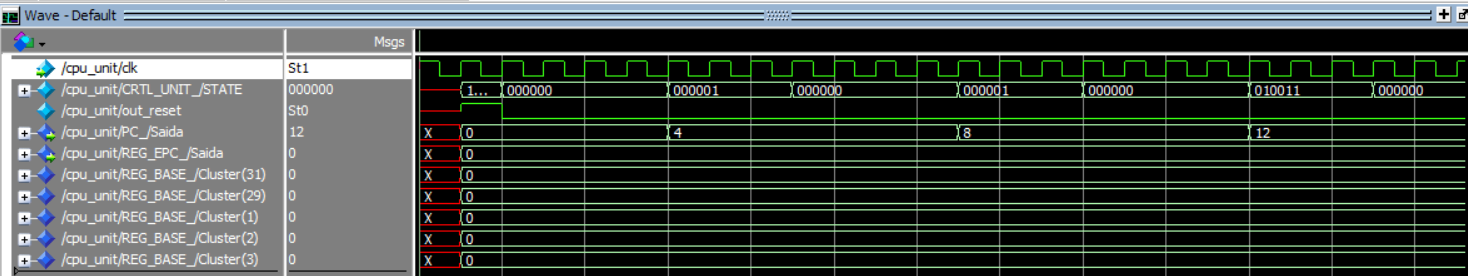
\includegraphics[width=1\textwidth]{figure/simulacao_and_neg.png}
\caption{Simulação And Neg} 
\label{fig:imagem_massa}
\end{figure}

\subsubsection{AND com resultado Positivo}
\textbf{Instruções testadas:} 
\lstinputlisting{codes/and_pos.asm} \\

\textbf{Descrição da simulação:} Será adicionado o valor 0 nos registradores \$1 e \$2 com o addi, os valores serão comparados e o resultado esperado é o valor 1 \\

\begin{figure}[htbp!]
\centering
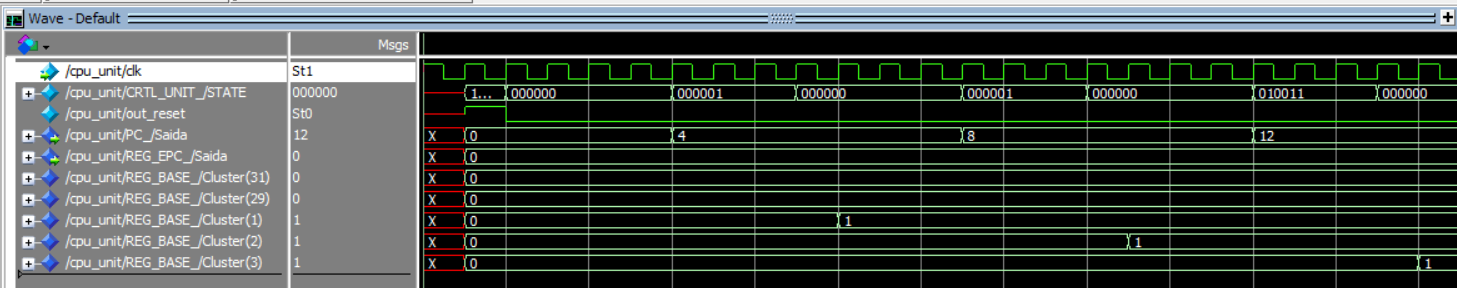
\includegraphics[width=1\textwidth]{figure/simulacao_and_pos.png}
\caption{Simulação And POS} 
\label{fig:imagem_massa}
\end{figure}
\newpage

\subsubsection{XCHG}
\textbf{Instruções testadas:}
\lstinputlisting{codes/xchg.asm} \\

\textbf{Descrição da simulação:} Será adicionado o valor 1 ao registrador \$1 e o valor 6 ao registrador \$2, e então os valores dos registradores 1 e 2 serão trocados.  \\

\begin{figure}[htbp!]
\centering
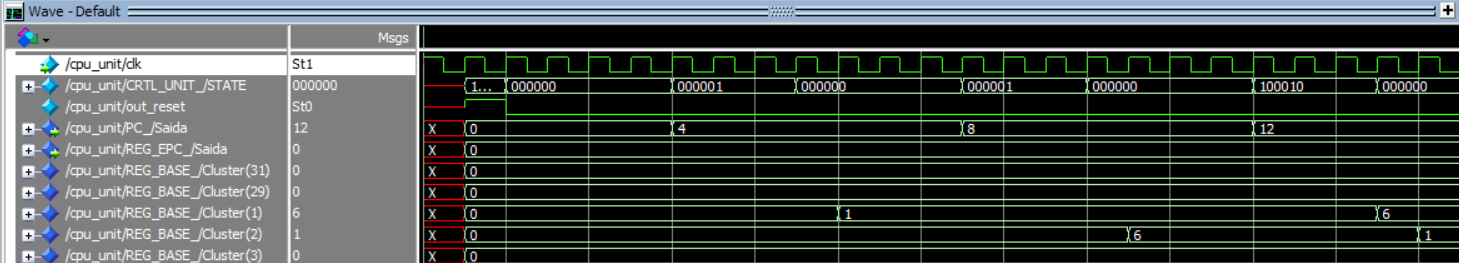
\includegraphics[width=1\textwidth]{figure/simulacao_xchg.png}
\caption{Simulação Xchg} 
\label{fig:imagem_massa}
\end{figure}


\subsubsection{BREAK}
\textbf{Instruções testadas:}
\lstinputlisting{codes/break.asm} \\

\textbf{Descrição da simulação:} Será adicionado o valor 1 no registrador \$1 e em seguida será adicionado a soma do valor do registrador \$1 com ele mesmo, resultando no valor 2. Então, a instrução break irá subtrair 4 do PC e entrará em loop com ela mesma. \\

\begin{figure}[htbp!]
\centering
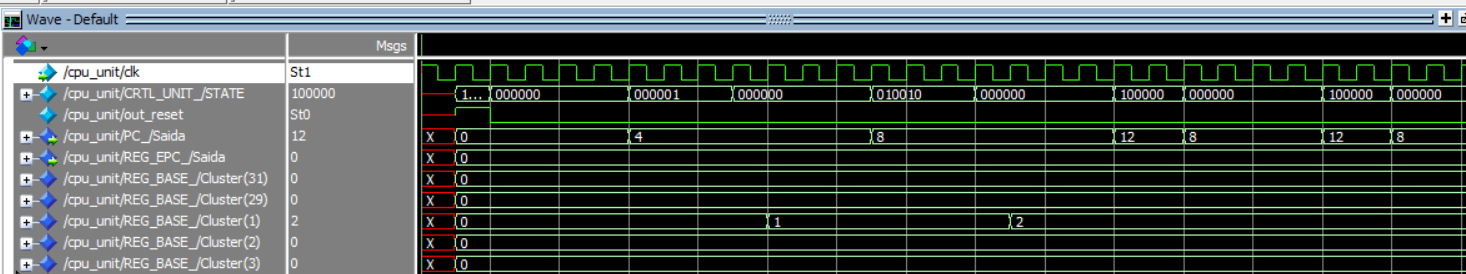
\includegraphics[width=1\textwidth]{figure/simulacao_break.png}
\caption{Simulação Break} 
\label{fig:imagem_massa}
\end{figure}

\newpage

\subsubsection{JR e JAL}
\textbf{Instruções testadas:}
\lstinputlisting{codes/jr_jal.asm} \\

\textbf{Descrição da simulação:} O valor 1 será adicionado ao registrador 1, e em seguida a instrução Jal (Jump and Link) salva o endereço da próxima instrução no registrador \$ra e salta para o endereço da etiqueta "pula". Em seguida, o valor 15 é adicionado ao registrador 1 resultando no valor 16. A instrução jr (jump register) vai para o endereço que está contido no registrador \$ra (linha 3) e soma o valor do registrador 1 com ele mesmo, resultando no valor 32. \\

\begin{figure}[htbp!]
\centering
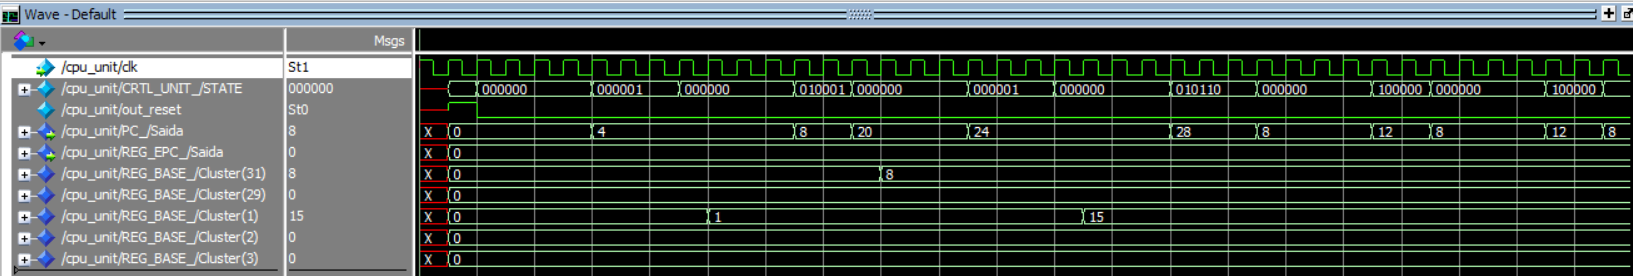
\includegraphics[width=1\textwidth]{figure/simulacao_jr_jal.png}
\caption{Simulação JR e JAL} 
\label{fig:imagem_massa}
\end{figure}

\subsubsection{MULT}
\textbf{Instruções testadas:}
\lstinputlisting{codes/mult.asm} \\

\textbf{Descrição da simulação:} O valor 72 é atribuído ao registrador \$1 e o valor 94 é atribuído ao registrador \$2. Em seguida, a instrução multiplica os dois valores, resultando no valor 6768. \\

\begin{figure}[htbp!]
\centering
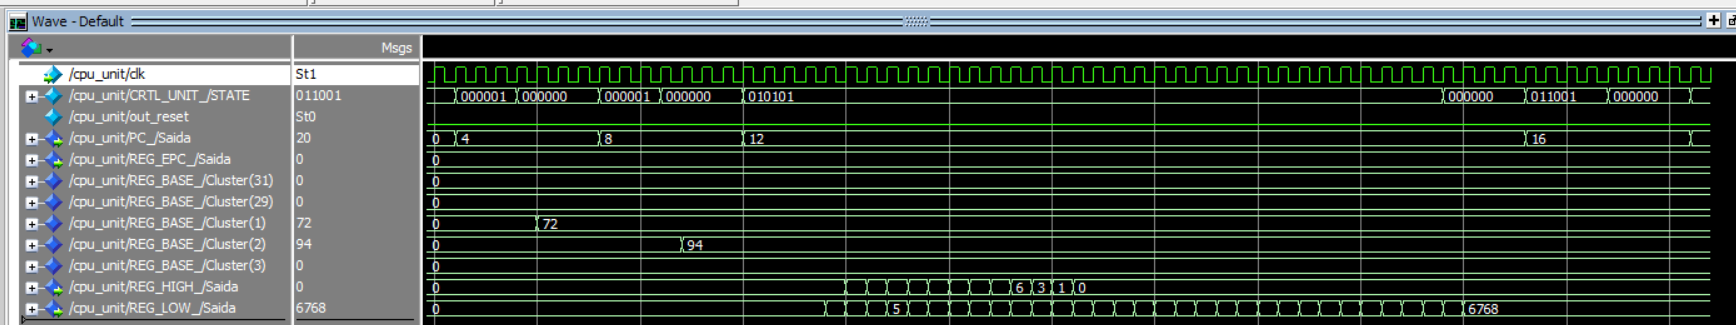
\includegraphics[width=1\textwidth]{figure/simulacao_mult.png}
\caption{Simulação Mult} 
\label{fig:imagem_massa}
\end{figure}

\newpage

\subsubsection{DIV}
\textbf{Instruções testadas:}
\lstinputlisting{codes/div.asm} \\

\textbf{Descrição da simulação:}  O valor 72 é atribuído ao registrador \$1 e o valor 5 é atribuído ao registrador \$2. Em seguida, a instrução divide os dois valores, o quociente 14 sendo armazenado no registrador HI e o resto 2 armazenado no registrador LO.   \\

\begin{figure}[htbp!]
\centering
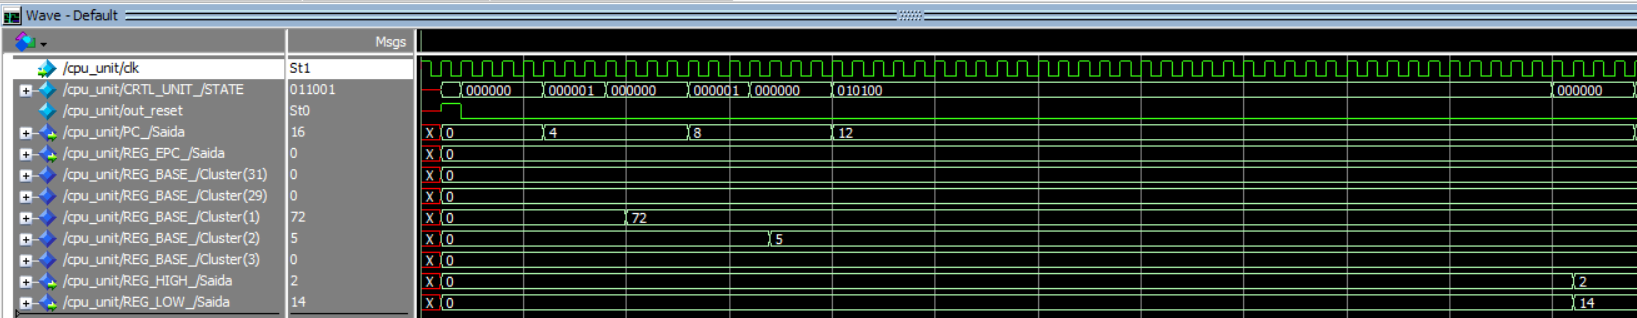
\includegraphics[width=1\textwidth]{figure/simulacao_div.png}
\caption{Simulação Div} 
\label{fig:imagem_massa}
\end{figure}

\subsubsection{MFHI e MFLO}
\textbf{Instruções testadas:}
\lstinputlisting{codes/mfhi_mflo.asm} \\

\textbf{Descrição da simulação:} O valor 13 é atribuído ao registrador \$1 e o valor 5 é atribuído ao registrador \$2. Em seguida, a instrução div divide o valor do registrador \$1 pelo do registrador \$2. A instrução mfhi atribui o valor 2 (que está armazenado no registrado HI) ao registrador \$3 e, em seguida, a instrução mflo atribui o valor 3 (que está armazenado no registrador LO) ao registrador \$3.\\

\begin{figure}[htbp!]
\centering
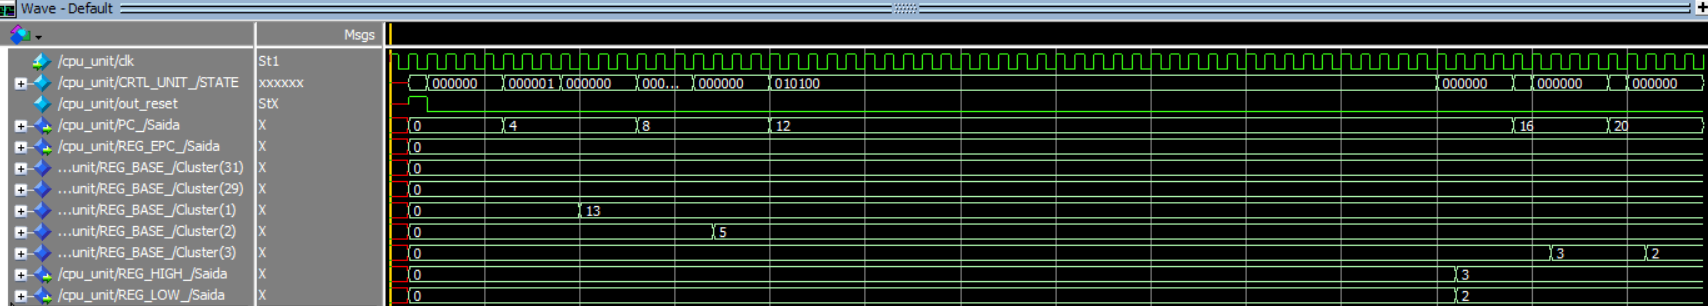
\includegraphics[width=1\textwidth]{figure/simulacao_mhfi_mflo.png}
\caption{Simulação Mhfi e Mflo} 
\label{fig:imagem_massa}
\end{figure}

\newpage

\subsubsection{SLL}
\textbf{Instruções testadas:}
\lstinputlisting{codes/sll.asm} \\

\textbf{Descrição da simulação:} A instrução addi adiciona o valor 2 ao registrador \$1 e em seguida a instrução sll realiza a operação de "Shift Left" por 8 bits no valor de \$1 e armazena o resultado (512) no registrador \$2. \\

\begin{figure}[htbp!]
\centering
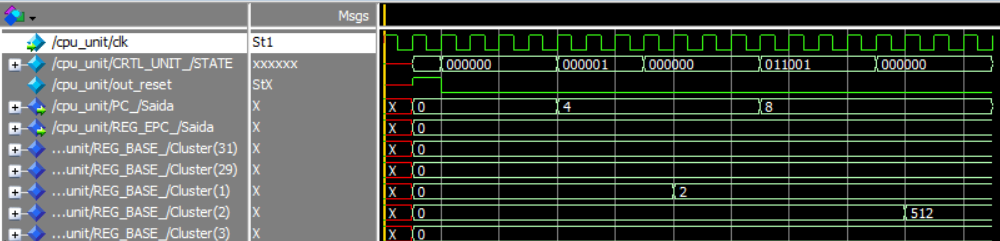
\includegraphics[width=1\textwidth]{figure/simulacao_sll.png}
\caption{Simulação Sll} 
\label{fig:imagem_massa}
\end{figure}


\subsubsection{SLLV}
\textbf{Instruções testadas:}
\lstinputlisting{codes/sllv.asm} \\

\textbf{Descrição da simulação:} A instrução addi é utilizada para adicionar o valor 2 a \$1 e em seguida adicionar o valor 8 a \$2. Então, a operação sllv (shift left logical variable) é utilizada para deslocar o valor de \$1 pelo número de bits especificado em \$2 e armazenar o resultado (512) em \$2.\\

\begin{figure}[htbp!]
\centering
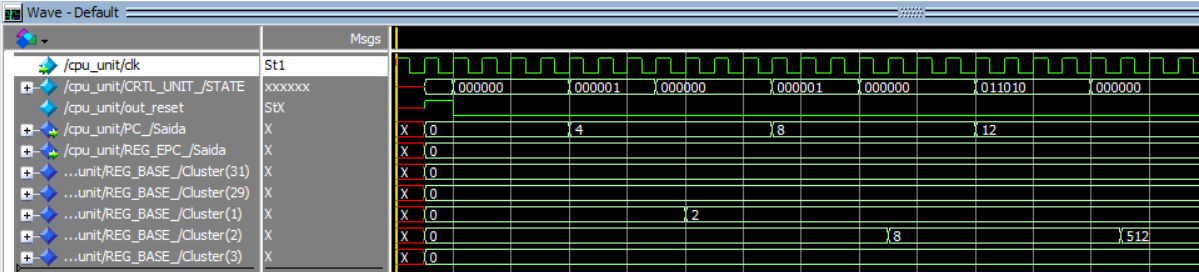
\includegraphics[width=1\textwidth]{figure/simulacao_sllv.png}
\caption{Simulação Sllv} 
\label{fig:imagem_massa}
\end{figure}

\newpage

\subsubsection{SLT}
\textbf{Instruções testadas:}
\lstinputlisting{codes/slt.asm} \\

\textbf{Descrição da simulação:} A instrução addi é utilizada para adicionar o valor 2 a \$1 e em seguida adicionar o valor 8 a \$2. Então, a operação slt (set less then) é utilizada para verificar se o valor no registrador \$1 é menor que o valor no registrador \$2. Se o valor de \$1 for menor que o de \$2, então \$3 receberá o valor 1, caso contrário, receberá o valor 0. Neste exemplo, como 2 é menor que 8, \$3 receberá o valor 1.  \\

\begin{figure}[htbp!]
\centering
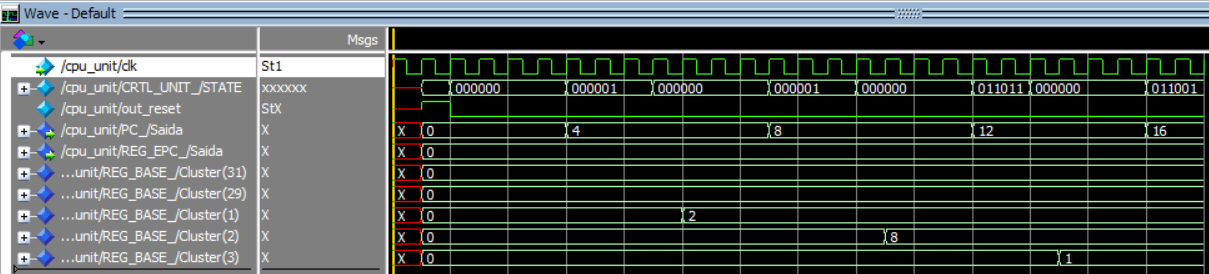
\includegraphics[width=1\textwidth]{figure/simulacao_slt.png}
\caption{Simulação SLT} 
\label{fig:imagem_massa}
\end{figure}

\subsubsection{SRA}
\textbf{Instruções testadas:}
\lstinputlisting{codes/sra.asm} \\

\textbf{Descrição da simulação:} A instrução addi é utilizada para adicionar o valor 8 a \$1, e então a operação sra (shif right arithmetic) é utilizada para deslocar o valor de \$1 em 2 bits para a direita (8 vira 2), armazenando o valor em \$3.  \\

\begin{figure}[htbp!]
\centering
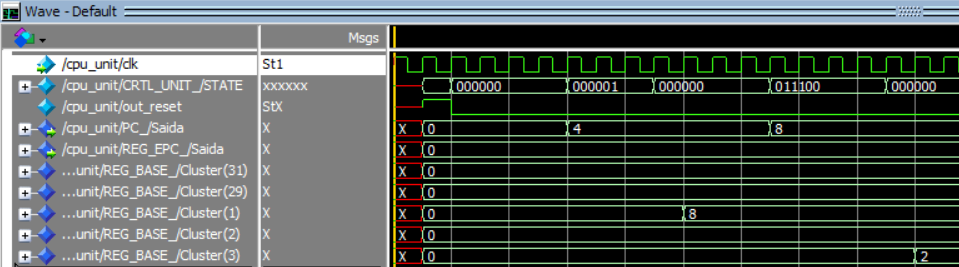
\includegraphics[width=1\textwidth]{figure/simulacao_sra.png}
\caption{Simulação SRA} 
\label{fig:imagem_massa}
\end{figure}

\newpage

\subsubsection{SRAV}
\textbf{Instruções testadas:}
\lstinputlisting{codes/srav.asm} \\

\textbf{Descrição da simulação:} A instrução addi é utilizada para adicionar o valor 8 a \$1 e em seguida adicionar o valor 2 a \$2. Então, a instrução srav (shift right arithmetic variable) realiza um deslocamento no registrador \$1 de acordo com o valor em \$2. Nesse exemplo, o resultado é 2.  \\

\begin{figure}[htbp!]
\centering
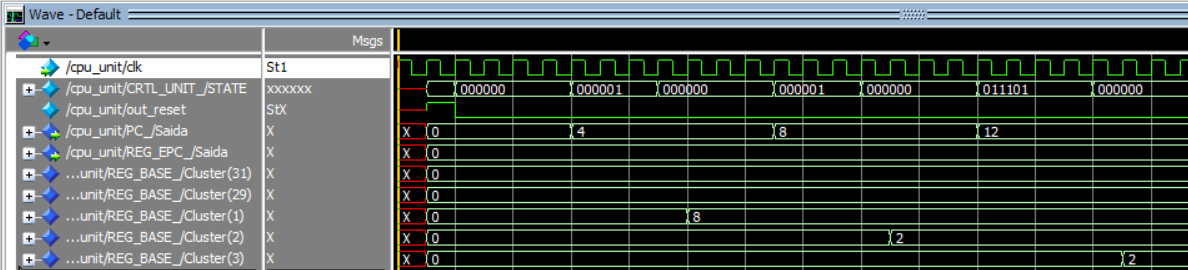
\includegraphics[width=1\textwidth]{figure/simulacao_srav.png}
\caption{Simulação SRAV} 
\label{fig:imagem_massa}
\end{figure}

\subsubsection{SRL}
\textbf{Instruções testadas:}
\lstinputlisting{codes/srl.asm} \\

\textbf{Descrição da simulação:} A instrução addi é utilizada para adicionar o valor 8 ao registrador \$1, e então a instrução srl (shift right logical) é utilizada para deslocar o valor de \$1 em 2 bits para a direita, neste exemplo o resultado seria 2. \\

\begin{figure}[htbp!]
\centering
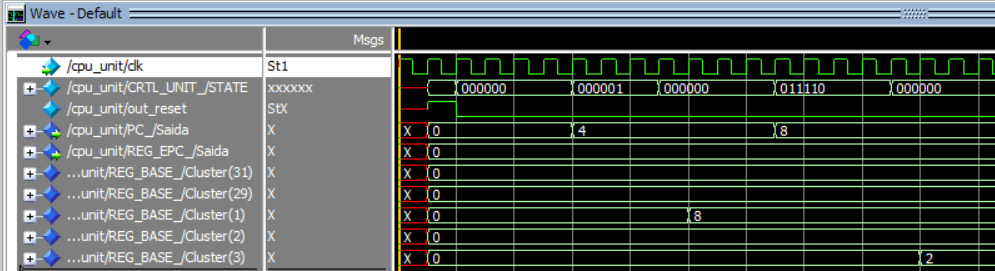
\includegraphics[width=1\textwidth]{figure/simulacao_srl.png}
\caption{Simulação SRL} 
\label{fig:imagem_massa}
\end{figure}

\newpage

\subsubsection{ADDI}
\textbf{Instruções testadas:}
\lstinputlisting{codes/addi.asm} \\

\textbf{Descrição da simulação:} A instrução addi é utilizada para adicionar o valor 8 ao registrador. \$1\\

\begin{figure}[htbp!]
\centering
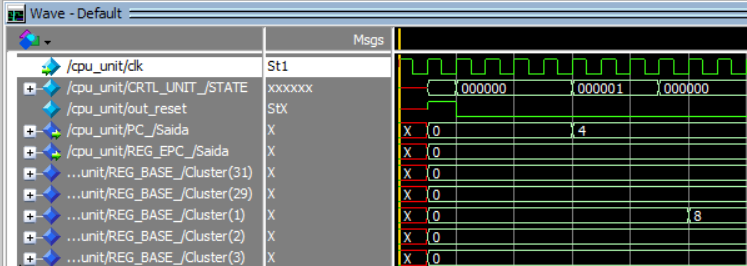
\includegraphics[width=1\textwidth]{figure/simulacao_addi.png}
\caption{Simulação ADDI} 
\label{fig:imagem_massa}
\end{figure}

\subsubsection{ADDIU}
\textbf{Instruções testadas:}
\lstinputlisting{codes/addiu.asm} \\

\textbf{Descrição da simulação:} A instrução addiu é utilizada para adicionar o valor 8 ao registrador \$1. Essa instrução é usingned, ou seja, quando o valor chega em um overflow, o resultado é o maior número que pode ser representado naquele limite.\\

\begin{figure}[htbp!]
\centering
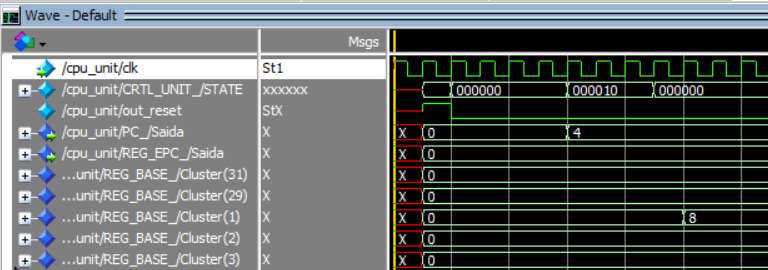
\includegraphics[width=1\textwidth]{figure/simulacao_addiu.png}
\caption{Simulação ADDIU} 
\label{fig:imagem_massa}
\end{figure}

\newpage

\subsubsection{BEQ com Desvio}
\textbf{Instruções testadas:}
\lstinputlisting{codes/beq_desvio.asm} \\

\textbf{Descrição da simulação:} A instrução addi é utilizada para atribuir o valor 8 aos registradores \$1 e \$2. Em seguida, a instrução beq (branch if equal) é utilizada para saltar para a label "LOOP" caso o valor dos registradores \$1 e \$2 forem iguais. Neste caso, eles são, então, a execução salta para a linha 7 e adiciona ao registrador \$3 o valor 99. \\

\begin{figure}[htbp!]
\centering
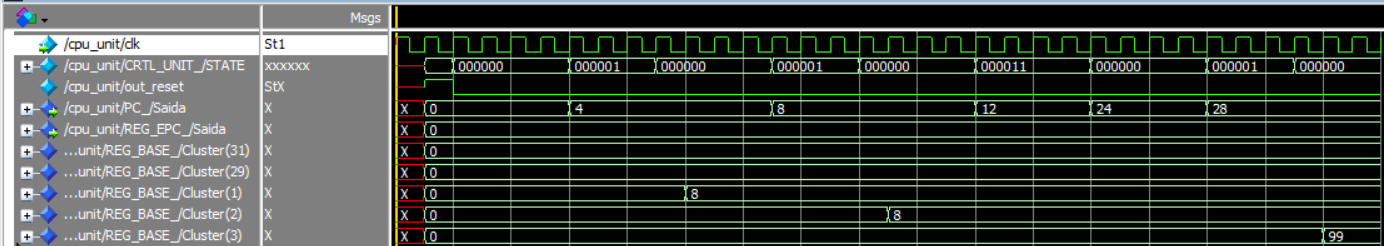
\includegraphics[width=1\textwidth]{figure/simulacao_beq_desvio.png}
\caption{Simulação BEQ com desvio} 
\label{fig:imagem_massa}
\end{figure}

\subsubsection{BEQ sem Desvio}
\textbf{Instruções testadas:}
\lstinputlisting{codes/beq_sem_desvio.asm} \\

\textbf{Descrição da simulação:} A instrução addi é utilizada para atribuir o valor 8 ao registrador \$1 e 9 ao registrador \$2. Em seguida, a instrução beq (branch if equal) é utilizada para saltar para a label "LOOP" caso o valor dos registradores \$1 e \$2 forem iguais. Neste caso, eles não são, então a execução continua e entra na execução do break, entrando em loop. \\

\begin{figure}[htbp!]
\centering
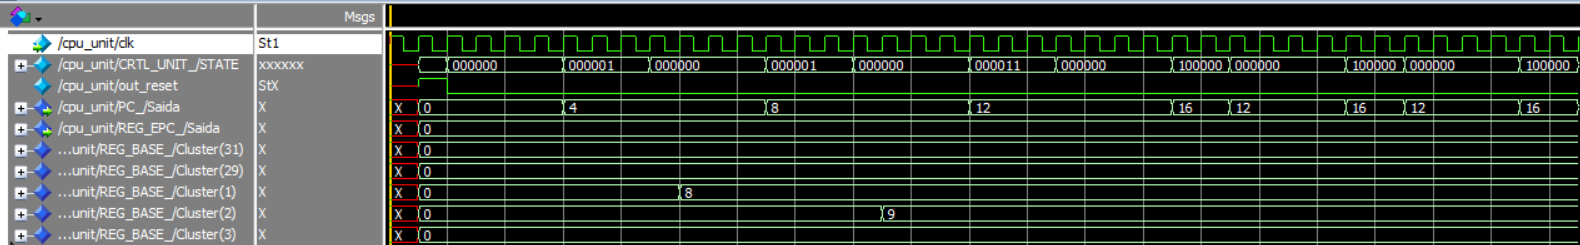
\includegraphics[width=1\textwidth]{figure/simulacao_beq_sem_desvio.png}
\caption{Simulação BEQ sem Desvio} 
\label{fig:imagem_massa}
\end{figure}

\subsubsection{BNE com Branch}
\textbf{Instruções testadas:}
\lstinputlisting{codes/bne_com_branch.asm} \\

\textbf{Descrição da simulação:} A instrução addi é utilizada para atribuir o valor 8 ao registrador \$1 e 9 ao registrador \$2. Em seguida, a instrução bne (branch if not equal) é utilizada para saltar para a label "LOOP" caso o valor dos registradores \$1 e \$2 não forem iguais. Neste caso, eles não são, então a execução salta para a linha 7 e adiciona ao registrador \$3 o valor 99. \\

\begin{figure}[htbp!]
\centering
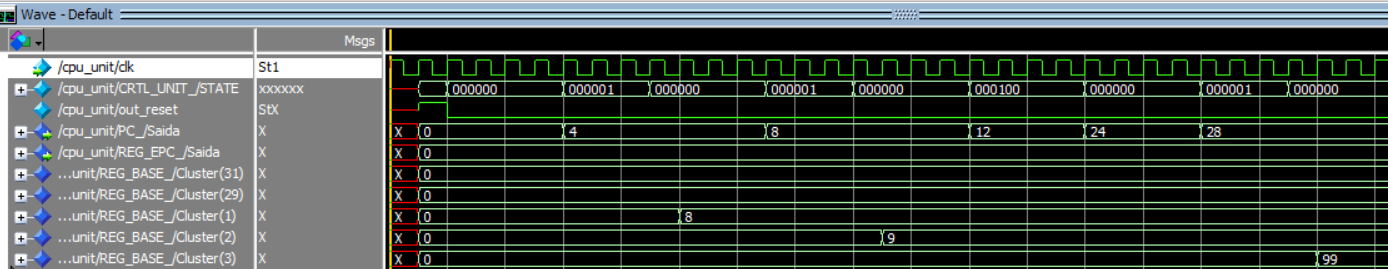
\includegraphics[width=1\textwidth]{figure/simulacao_bne_com_branch.png}
\caption{Simulação BNE com Branch} 
\label{fig:imagem_massa}
\end{figure}

\subsubsection{BNE sem Branch}
\textbf{Instruções testadas:}
\lstinputlisting{codes/bne_sem_branch.asm} \\

\textbf{Descrição da simulação:} A instrução addi é utilizada para atribuir o valor 9 aos registradores \$1 e \$2. Em seguida, a instrução bne (branch if not equal) é utilizada para saltar para a label "LOOP" caso o valor dos registradores \$1 e \$2 não forem iguais. Neste caso, eles são, então, a execução continua entrando no break e seguindo no loop.\\

\begin{figure}[htbp!]
\centering
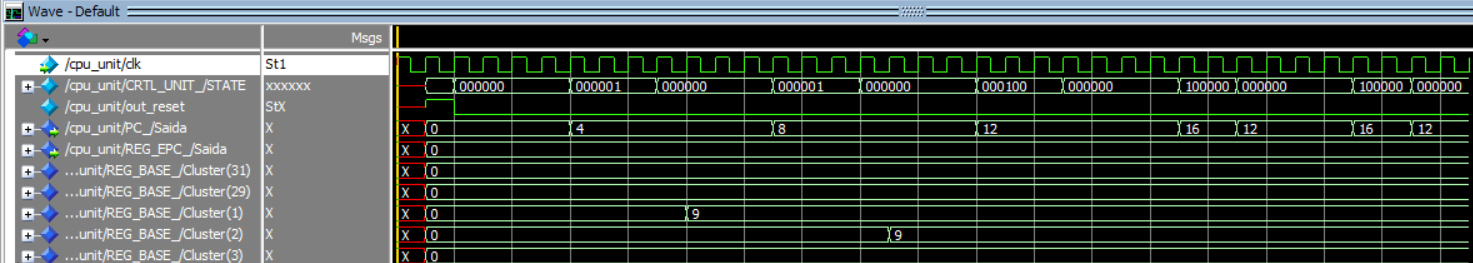
\includegraphics[width=1\textwidth]{figure/simulacao_bne_sem_branch.png}
\caption{Simulação BNE sem Branch} 
\label{fig:imagem_massa}
\end{figure}

\subsubsection{BLE com Branch}
\textbf{Instruções testadas:}
\lstinputlisting{codes/ble_com_branch.asm} \\

\textbf{Descrição da simulação:} A instrução addi é utilizada para atribuir o valor 1 ao registrador \$1 e 2 a \$2. Em seguida, a instrução ble (branch if less than or equal to) é utilizada para comparar os valores de \$1 e \$2 e enviar o programa para a label "LOOP". Como 1 é menor ou igual a 2, então o programa vai para a linha 7 e adiciona o valor 99 ao registrador \$3.\\

\begin{figure}[htbp!]
\centering
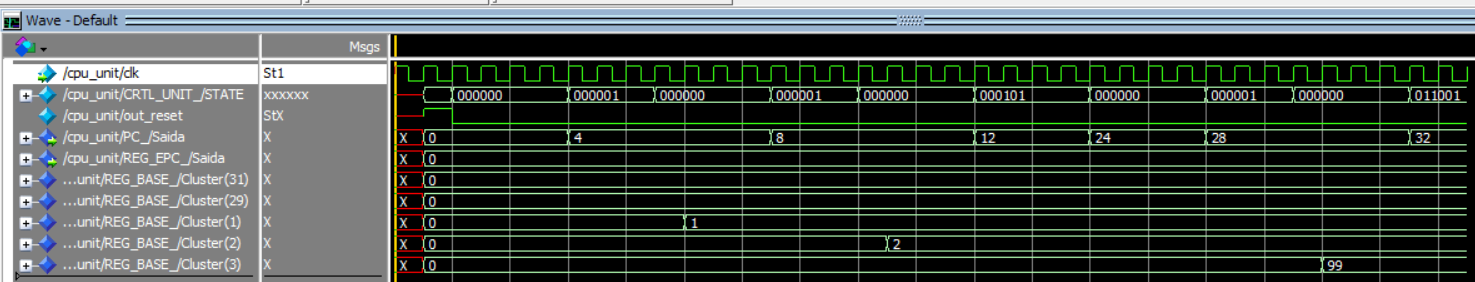
\includegraphics[width=1\textwidth]{figure/simulacao_ble_com_branch.png}
\caption{Simulação BLE com Branch} 
\label{fig:imagem_massa}
\end{figure}

\subsubsection{BLE sem Branch}
\textbf{Instruções testadas:}
\lstinputlisting{codes/ble_sem_branch.asm} \\

\textbf{Descrição da simulação:} A instrução addi é utilizada para atribuir o valor 1 ao registrador \$1 e 2 a \$2. Em seguida, a instrução ble (branch if less than or equal to) é utilizada para comparar os valores de \$2 e \$1 e enviar o programa para a label "LOOP". Como 2 é maior que 1, então o programa segue e entra no break, não saindo mais dessa instrução. \\

\begin{figure}[htbp!]
\centering
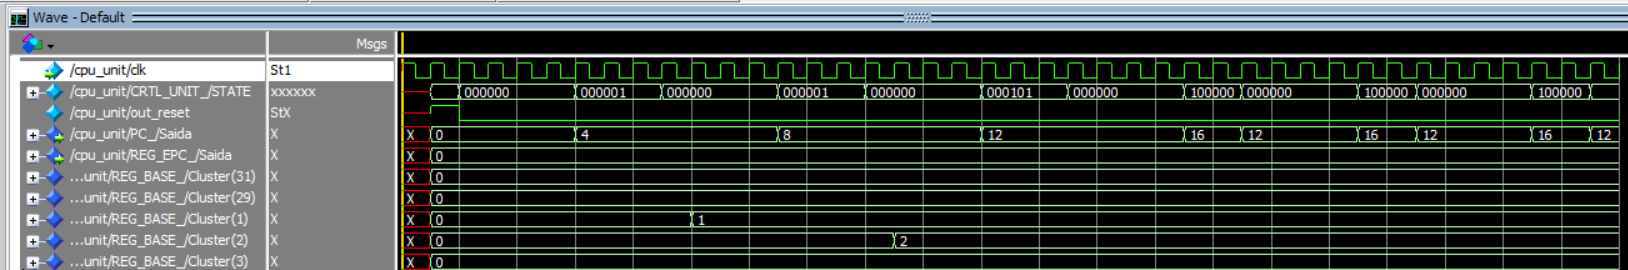
\includegraphics[width=1\textwidth]{figure/simulacao_ble_sem_branch.png}
\caption{Simulação BLE sem Branch} 
\label{fig:imagem_massa}
\end{figure}

\subsubsection{BGT com Branch}
\textbf{Instruções testadas:}
\lstinputlisting{codes/bgt_com_branch.asm} \\

\textbf{Descrição da simulação:} A instrução addi é utilizada para atribuir o valor 1 ao registrador \$1 e 2 ao registrador \$2. Em seguida, a instrução bgt (branch if greater than) verifica se o valor de \$2 é maior que o valor de \$1. Neste caso, como 2 é maior que 1 então o código pula para a label "LOOP" na linha 7, adicionando o valor 99 ao registrador \$3.\\

\begin{figure}[htbp!]
\centering
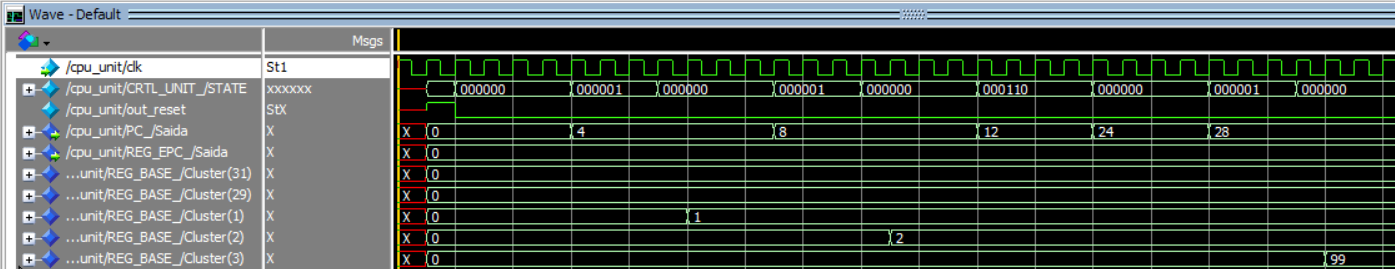
\includegraphics[width=1\textwidth]{figure/simulacao_bgt_com_branch.png}
\caption{Simulação BGT com Branch} 
\label{fig:imagem_massa}
\end{figure}

\newpage

\subsubsection{BGT sem Branch}
\textbf{Instruções testadas:}
\lstinputlisting{codes/bgt_sem_branch.asm} \\

\textbf{Descrição da simulação:} A instrução addi é utilizada para atribuir o valor 1 ao registrador \$1 e 2 ao registrador \$2. Em seguida, a instrução bgt (branch if greater than) verifica se o valor de \$1 é maior que o valor de \$2. Neste caso, como 1 não é maior que 2 então o código continua normalmente, entrando na instrução break e rodando ela infinitamente.\\

\begin{figure}[htbp!]
\centering
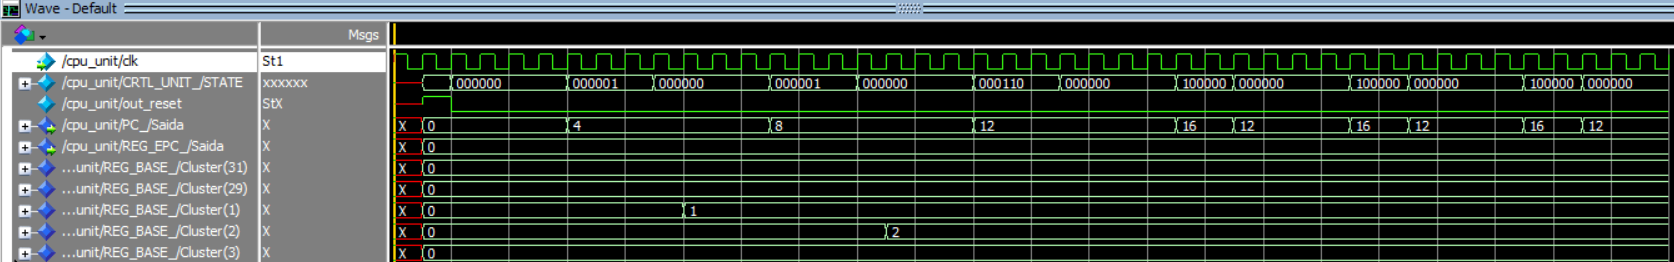
\includegraphics[width=1\textwidth]{figure/simulacao_bgt_sem_branch.png}
\caption{Simulação BGT sem Branch} 
\label{fig:imagem_massa}
\end{figure}

\newpage

\subsubsection{SRAM}
\textbf{Instruções testadas:}
\lstinputlisting{codes/sram.asm} \\

\textbf{Descrição da simulação:} A instrução addi é utilizada para adicionar o valor 1023 ao registrador \$2, o valor -1023 ao registrador \$3 e 5 ao registrador \$4. Então, a instrução sw armazenazena o valor de \$4 na memória 100 bytes após o endereço de \$10. Após isso a instrução sw passa para o registrador \$2 o conteúdo desse endereço de memória. Então, o sram desloca o valor do registrador 2, na quantidade de bits contida no endereço de memória.  \\

\begin{figure}[htbp!]
\centering
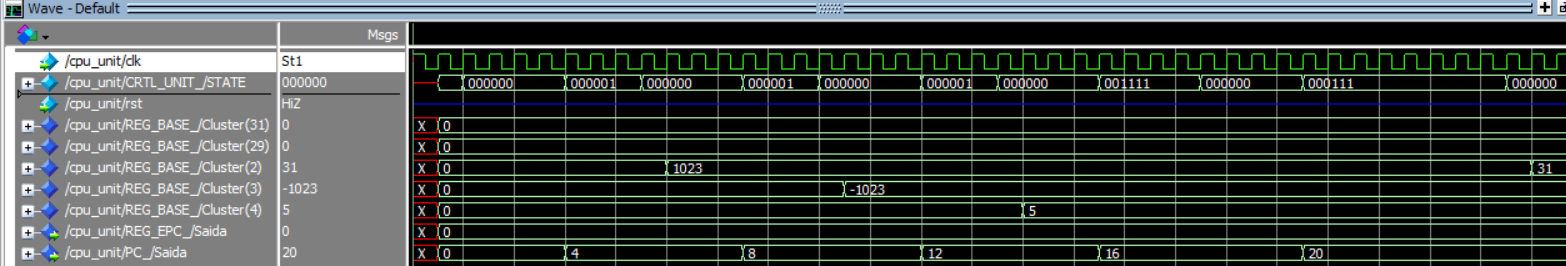
\includegraphics[width=1\textwidth]{figure/simulacao_sram.png}
\caption{Simulação SRAM} 
\label{fig:imagem_massa}
\end{figure}

\subsubsection{LW}
\textbf{Instruções testadas:}
\lstinputlisting{codes/lw.asm} \\

\textbf{Descrição da simulação:} A instrução lui é utilizada para adicionar o shift left 16 do valor 32767 no registrador \$2, e addi é utilizada para adcionar o para somar 32639 ao valor do do registrador \$2 em seguida sw armazena o valor de \$2 na posição de memória 140(\$10). Então, a instrução lw carrega o valor o valor da posição de memória 140(\$10) no registrador \$3.\\

\begin{figure}[htbp!]
\centering
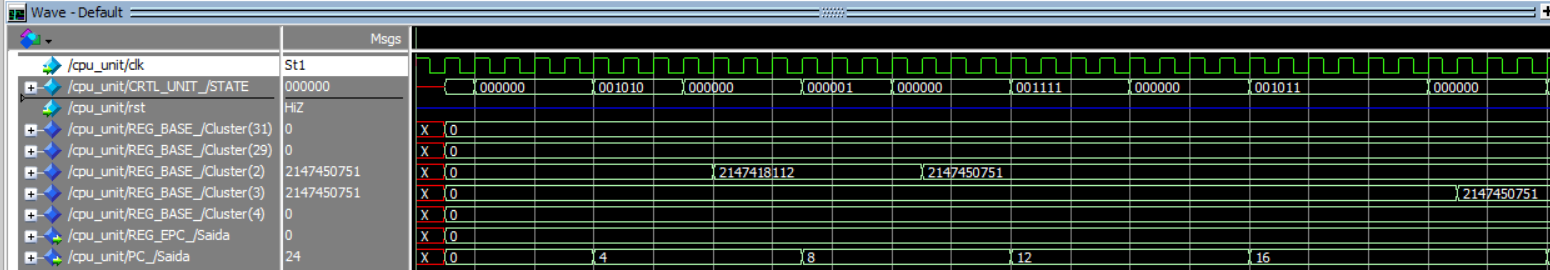
\includegraphics[width=1\textwidth]{figure/simulacao_lw.png}
\caption{Simulação LW} 
\label{fig:imagem_massa}
\end{figure}

\newpage
\subsubsection{LB e LH}
\textbf{Instruções testadas:}
\lstinputlisting{codes/lb_lh.asm} \\

\textbf{Descrição da simulação:} A instrução lui é utilizada para adicionar o shift left 16 do valor 32767 ao registrador \$2 e addi é utilizada para adicionar o valor 32639 ao registrador \$2. Em seguida, a instrução sw armazena o valor de \$2 na posição de memória 140(\$10), a instrução lw carrega no registrador \$3 o valor de 140(\$10) a instrução lb carrega uma meia palavra (2 bytes) da posição de memória 140(\$10) no o registrador \$4 e então a instrução lb carrega um byte de 140(\$10) no registrador \$5.  \\

\begin{figure}[htbp!]
\centering
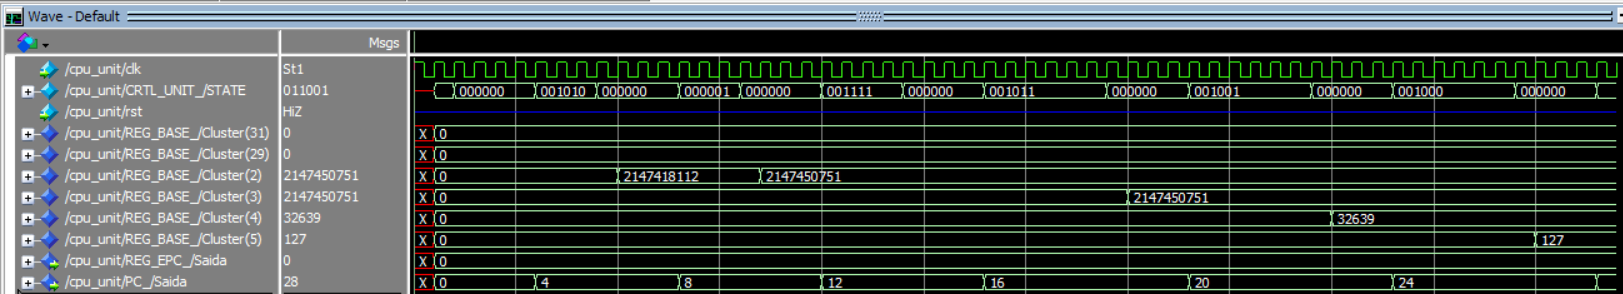
\includegraphics[width=1\textwidth]{figure/simulacao_lb_lh.png}
\caption{Simulação LB e LH} 
\label{fig:imagem_massa}
\end{figure}

\subsubsection{SW, SH e SB}
\textbf{Instruções testadas:}
\lstinputlisting{codes/sw_sh_sb.asm} \\

\textbf{Descrição da simulação:} A instrução lui é utilizada para adicionar o shift left 16 do valor 32767 ao registrador \$2, addi é utilizada para adicionar o valor 32639 ao registrador \$2. Em seguida as instruções sw, sh e sb armazenam respectivamente os valores \$2, os 16 bits menos significativos de \$2 e o byte menos signicativo de \$2 nos endereços de memória  100(\$10), 108(\$10) e 116(\$10) e as 3 ultimas instruções carregam os valores dessas posições de memória nos registradores \$3, \$4 e \$5 para podermos analisar os resultados.\\

\begin{figure}[htbp!]
\centering
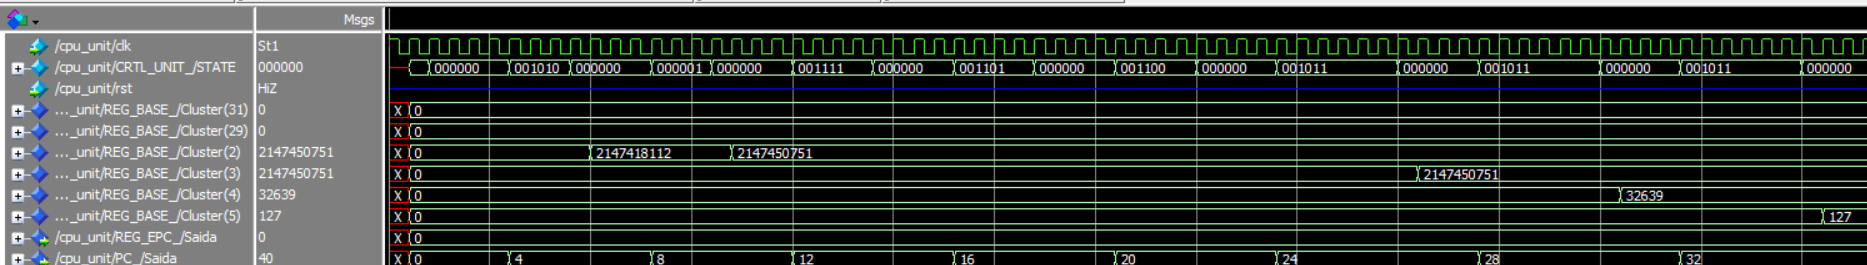
\includegraphics[width=1\textwidth]{figure/simulacao_sw_sh_sb.png}
\caption{Simulação SW, SH e SB} 
\label{fig:imagem_massa}
\end{figure}

\subsubsection{ADDIU Overflow}
\textbf{Instruções testadas:}
\lstinputlisting{codes/addiu_com_overflow.asm} \\

\textbf{Descrição da simulação:} A instrução lui é utilizada para adicionar o shift left 16 do valor 32767 ao registrador \$2, addi é utilizado duas vezes para adicionar o valor 32767 ao registrador \$2 e addi é utilizado para adicionar o valor 1 a \$2. Então add é utilizado para adicionar somar o valor dos registradores \$0 (zero) e \$2 e armazenar em \$3. Aqui \$2 e \$3 possuem o mesmo valor. Em seguida addiu é utilizado para somar 1 ao registrador \$2 e addi é utilizado para somar 1 ao registrador \$3. Podemos perceber que somar 1 com o addiu, não ocorre overflow, mas ao somar 1 com o add este problema ocorre. \\

\begin{figure}[htbp!]
\centering
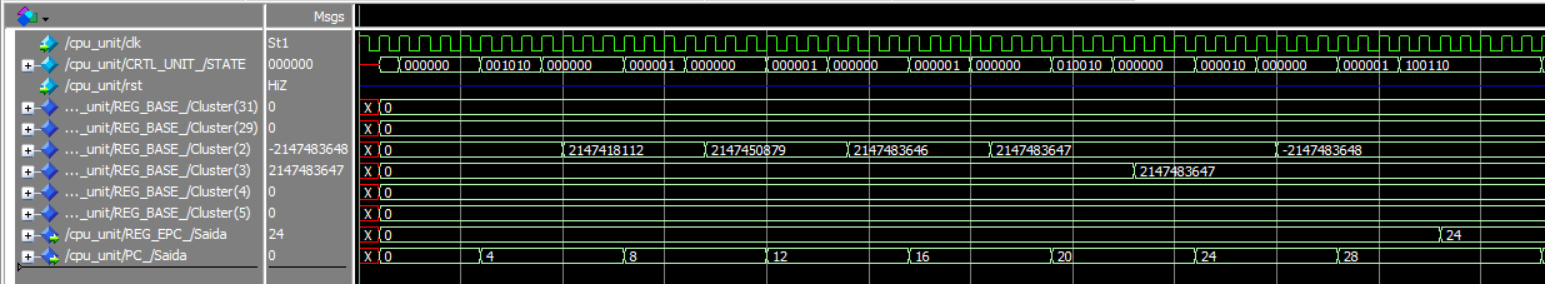
\includegraphics[width=1\textwidth]{figure/simulacao_addiu_com_overflow.png}
\caption{Simulação ADDIU com Overflow} 
\label{fig:imagem_massa}
\end{figure}

\subsubsection{Error Div 0}
\textbf{Instruções testadas:}
\lstinputlisting{codes/div0.asm} \\

\textbf{Descrição da simulação:} A instrução addi é utilizada para armazenar o valor 5 no registrador \$2 e depois a instruçao div divide 0 por 0, pode-se ver então que o valor da flag zero em CRTL\_UNIT\_ZERO\_/zero vira 1 e o erro é tratado.\\

\newpage

\begin{figure}[htbp!]
\centering
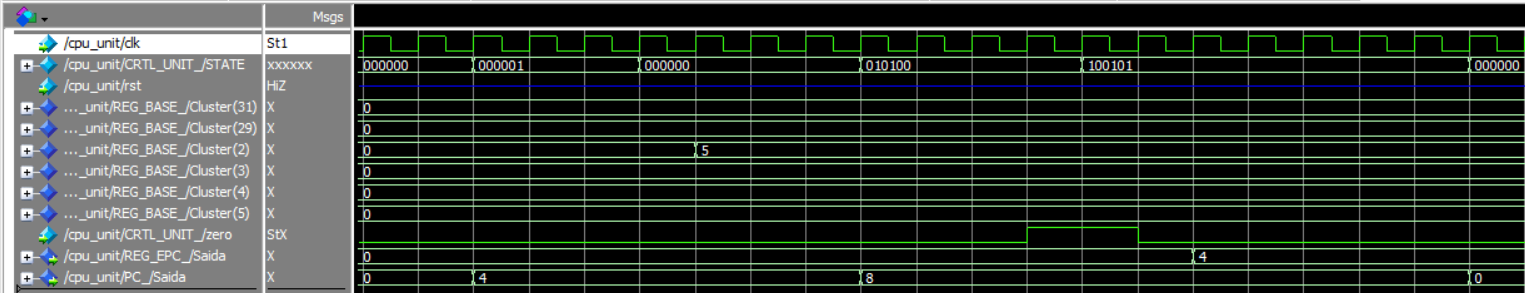
\includegraphics[width=1\textwidth]{figure/simulacao_div_por_zero.png}
\caption{Simulação Error Div 0} 
\label{fig:imagem_massa}
\end{figure}

\subsubsection{Overflow}
\textbf{Instruções testadas:} 
\lstinputlisting{codes/overflow.asm} \\

\textbf{Descrição da simulação:} A instrução lui é utilizada para adicionar o shift left 16 do valor 32767 ao registrador \$2. Então, a instrução addi é utilizada duas vezes para adicionar o valor 32767 ao registrador \$3 e em seguida addi é utilizada para adicionar o valor 2 a \$3, ocorrendo overflow.  \\

\begin{figure}[htbp!]
\centering
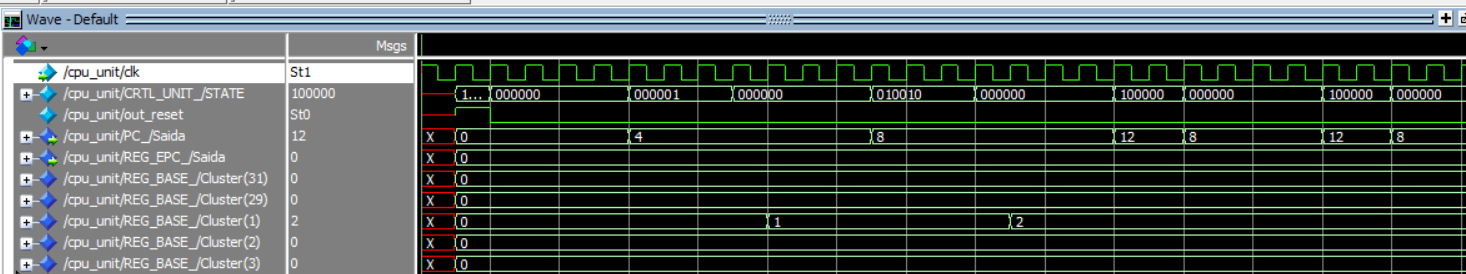
\includegraphics[width=1\textwidth]{figure/simulacao_break.png}
\caption{Simulação Overflow} 
\label{fig:imagem_massa}
\end{figure}

\subsubsection{Operror}
\textbf{Instruções testadas:}
\lstinputlisting{codes/operror.asm} \\

\textbf{Descrição da simulação:} A instrução lui é utilizada para adicionar o shift left 16 do valor 32767 ao registrador \$2 e então é chamada a instrução null, que não contém um OPCODE válido, resultando em OPERROR.\\

\begin{figure}[htbp!]
\centering
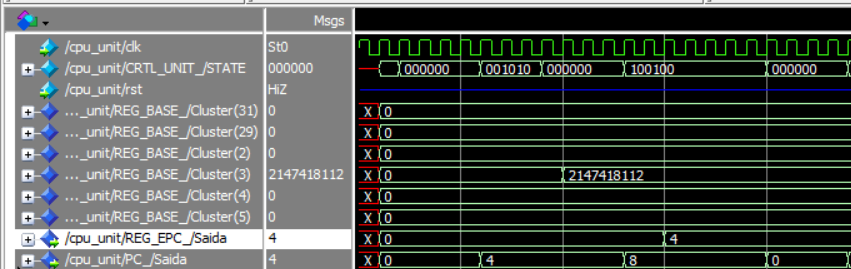
\includegraphics[width=1\textwidth]{figure/simulacao_operror.png}
\caption{Simulação Operror} 
\label{fig:imagem_massa}
\end{figure}

\newpage
\subsubsection{J}
\textbf{Instruções testadas:}
\lstinputlisting{codes/j.asm} \\

\textbf{Descrição da simulação:} A instrução J pula a sequencia do código para a flag LOOP e a instrução addi da flag LOOP armazena 30 no registrador \$2. \\

\begin{figure}[htbp!]
\centering
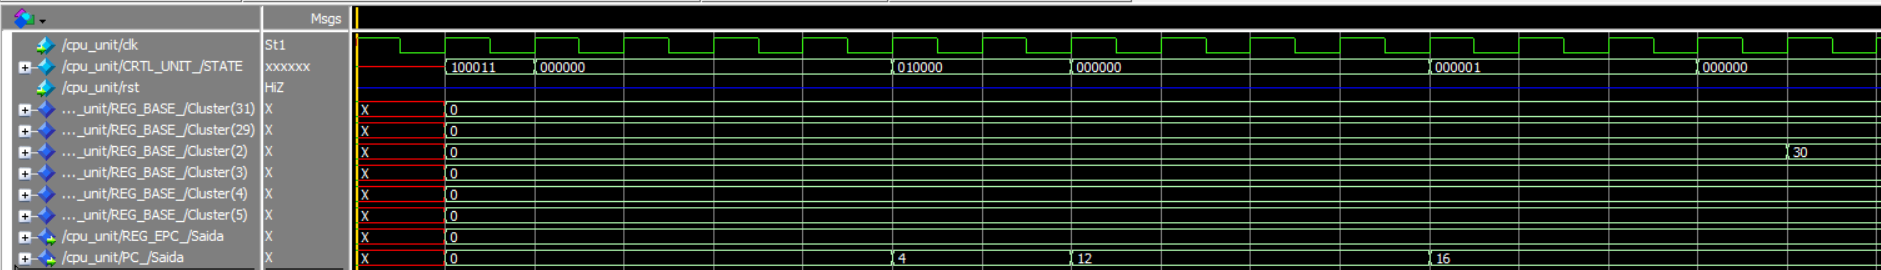
\includegraphics[width=1\textwidth]{figure/simulacao_j.png}
\caption{Simulação J} 
\label{fig:imagem_massa}
\end{figure}

\subsubsection{LUI}
\textbf{Instruções testadas:}
\lstinputlisting{codes/lui.asm} \\

\textbf{Descrição da simulação:} A instrução LUI é utilizada para adicionar o shift left 16 do valor 32767 no registrador \$3, como podemos ver o valor armazenado é 2147418112, equivalente a $32767*2^{16}$. \\

\begin{figure}[htbp!]
\centering
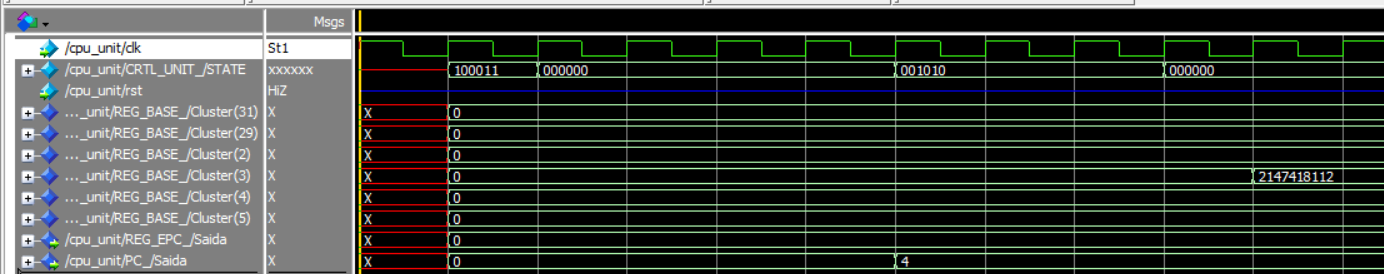
\includegraphics[width=1\textwidth]{figure/simulacao_lui.png}
\caption{Simulação LUI} 
\label{fig:imagem_massa}
\end{figure}

\newpage
\subsubsection{RTE}
\textbf{Instruções testadas:}
\lstinputlisting{codes/rte.asm} \\

\textbf{Descrição da simulação:} A instrução lui é utilizada para adicionar o shift left 16 do valor 32767 ao registrador \$3, addi é utilizado para adicionar o valor 12 ao registrador \$2 então a instrução rte é lida que armazena o valor de epc em pc, nesse caso o valor de epc era 0 então podemos ver que PC\_/saida vira 0.  \\

\begin{figure}[htbp!]
\centering
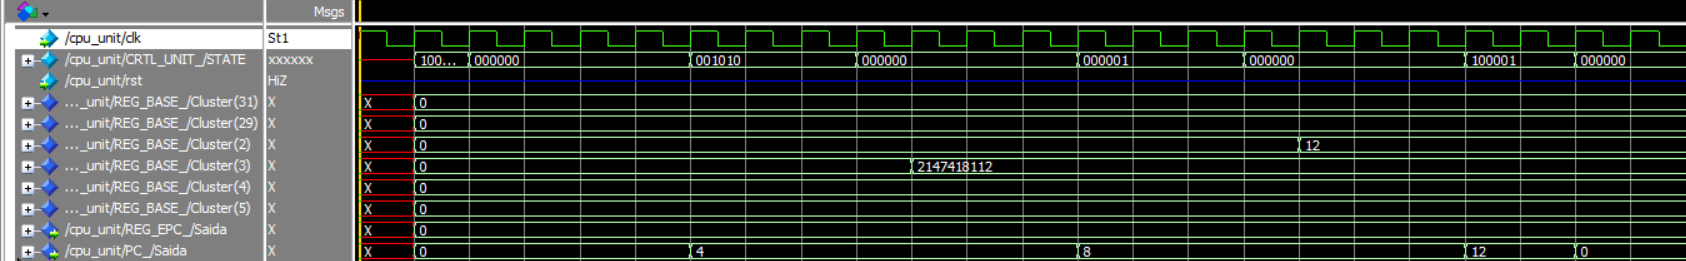
\includegraphics[width=1\textwidth]{figure/simulacao_rte.png}
\caption{Simulação RTE} 
\label{fig:imagem_massa}
\end{figure}


\newpage


\section{Conclusão}

Desenvolver uma CPU é uma tarefa desafiadora que exige um profundo entendimento dos princípios de arquitetura de computadores e design de hardware. Ao concluir este projeto, ficou claro que a implementação de uma CPU requer não apenas competências técnicas, mas também uma compreensão abrangente dos circuitos lógicos subjacentes e dos protocolos de comunicação. Através deste processo, foi possível explorar e aprimorar nossas habilidades em design de hardware, desde a concepção inicial até a depuração e otimização do código de baixo nível. Este projeto proporcionou uma experiência valiosa na aplicação prática de conceitos teóricos de arquitetura de computadores, consolidando o conhecimento para compreender o funcionamento de processadores e enfrentar desafios futuros na área de infraestrutura e design de processadores.
